%%%%%%%%%%%%%%%%%%%%%%%%%%%%%%%%%%%%%%%%%%%%%%%%%%%%%%%%%%%%%%%%%%%%
%% I, the copyright holder of this work, release this work into the
%% public domain. This applies worldwide. In some countries this may
%% not be legally possible; if so: I grant anyone the right to use
%% this work for any purpose, without any conditions, unless such
%% conditions are required by law.
%%%%%%%%%%%%%%%%%%%%%%%%%%%%%%%%%%%%%%%%%%%%%%%%%%%%%%%%%%%%%%%%%%%%

\documentclass[
  digital, %% This option enables the default options for the
           %% digital version of a document. Replace with `printed`
           %% to enable the default options for the printed version
           %% of a document.
  notable,   %% Causes the coloring of tables. Replace with `notable`
           %% to restore plain tables.
  nolof,     %% Prints the List of Figures. Replace with `nolof` to
           %% hide the List of Figures.
  nolot,     %% Prints the List of Tables. Replace with `nolot` to
           %% hide the List of Tables.
%   draft
  %% More options are listed in the user guide at
  %% <http://mirrors.ctan.org/macros/latex/contrib/fithesis/guide/mu/fi.pdf>.
]{fithesis3}
%% The following section sets up the locales used in the thesis.
\usepackage[resetfonts]{cmap} %% We need to load the T2A font encoding
\usepackage[T1,T2A]{fontenc}  %% to use the Cyrillic fonts with Russian texts.
\usepackage[
  main=english, %% By using `czech` or `slovak` as the main locale
                %% instead of `english`, you can typeset the thesis
                %% in either Czech or Slovak, respectively.
  %english, german, russian, czech, slovak %% The additional keys allow
]{babel}        %% foreign texts to be typeset as follows:
%%
%%   \begin{otherlanguage}{german}  ... \end{otherlanguage}
%%   \begin{otherlanguage}{russian} ... \end{otherlanguage}
%%   \begin{otherlanguage}{czech}   ... \end{otherlanguage}
%%   \begin{otherlanguage}{slovak}  ... \end{otherlanguage}
%%
%% For non-Latin scripts, it may be necessary to load additional
%% fonts:
\usepackage{paratype}
\usepackage{textcomp} % to be able to use normal apostrophe with \textquotesingle
\def\textrussian#1{{\usefont{T2A}{PTSerif-TLF}{m}{rm}#1}}
%%
%% The following section sets up the metadata of the thesis.
\thesissetup{
    date          = 2018/05/20,
    university    = mu,
    faculty       = fi,
    type          = mgr,
    author        = {Jiří Mauritz},
    gender        = m,
    advisor       = {RNDr. Zuzana Nevěřilová, Ph.D.}, 
    title         = {Automatic Classification of Legal Documents},
    TeXtitle      = {Automatic Classification of Legal Documents},
    keywords      = {machine learning, legal documents, natural language processing},
    TeXkeywords   = {machine learning, legal documents, natural language processing},
    abstract      = {This is the abstract of my thesis, which can

                     span multiple paragraphs.},
    thanks        = {These are the acknowledgements for my thesis, which can

                     span multiple paragraphs.},
    bib           = example.bib,
}
\usepackage{makeidx}      %% The `makeidx` package contains
\makeindex                %% helper commands for index typesetting.
%% These additional packages are used within the document:
\usepackage{paralist} %% Compact list environments
\usepackage{amsmath}  %% Mathematics
\usepackage{amsthm}
\usepackage{amsfonts}
\usepackage{url}      %% Hyperlinks
\usepackage{markdown} %% Lightweight markup
\usepackage{listings} %% Source code highlighting
\lstset{
  basicstyle      = \ttfamily,%
  identifierstyle = \color{black},%
  keywordstyle    = \color{blue},%
  keywordstyle    = {[2]\color{cyan}},%
  keywordstyle    = {[3]\color{olive}},%
  stringstyle     = \color{teal},%
  commentstyle    = \itshape\color{magenta}}
\usepackage{floatrow} %% Putting captions above tables
\usepackage{slashbox} %% Big slash in tables
\usepackage{cleveref}[2012/02/15] %% Enables cross reference footnotes
\floatsetup[table]{capposition=top}
\usepackage{minted} % nice listings
%\usemintedstyle{fruity}
\usepackage{amsmath,amssymb} % math
\DeclareRobustCommand{\bbone}{\text{\usefont{U}{bbold}{m}{n}1}}
\DeclareMathOperator{\EX}{\mathbb{E}}% expected value
\usepackage[table]{xcolor}
\usepackage{subcaption}

\begin{document}
\chapter*{Introduction}
\addcontentsline{toc}{chapter}{Introduction}

introduction

\chapter{Related work}
This chapter summarizes the previous work on the application of artificial intelligence in the legal domain. 
The first section describes a general role of artificial intelligence in law and how it evolved in time.
Researchers in this field focused mainly on decision-making systems to support work of the jury; however, this research focuses more on the information retrieval and knowledge discovery in the legal domain, also known as \textit{Electronic Discovery}, which brings a support for lawyers.
Therefore, the second section looks more closely at this subfield by introducing state-of-the-art legal retrieval systems and underlines common characteristics with the research presented here.
The last section discusses an issue of relevance in the legal context and related studies.

\section{Artificial Intelligence and Law}
The global publishing company \textit{Springer} introduced a journal \textit{Artificial Intelligence and Law} \footnote{\url{https://link.springer.com/journal/10506}} in 1992 which contains 426 published articles (as of March 2018) describing theoretical and empirical studies in artificial intelligence (AI) from the legal perspective.
Though the journal consists of articles concerned with AI as a new trend that needs to be bound by law, such as legal aspects of autonomous vehicles \cite{Prakken2017autonomous}, robot sex \cite{Frank2017robotSex} or responsibility of autonomous machines \cite{Brozek2017AIresponsibility}, it also contains researches of new innovative AI systems that perform automatic reasoning and knowledge extraction in the legal domain.
The collection of AI-law related articles provides enough information to create a brief overview of how this field has evolved over time.

The first legal search engines enabled retrieving results by first-order logic rules and fixed pieces of text \cite{Turtle1995legalRetrieval}.
In the early 1990s, the concept of full-text search has become widely used and users could enjoy a retrieval by a plain natural language \cite{Turtle1995legalRetrieval}.
Shortly after, researchers started to focus on AI when creating a new legal retrieval system, such as legal text management system \textit{Flexlaw} (\citeyear{Smith1995flexlaw}) \cite{Smith1995flexlaw}, integrated decision support system \textit{DataLex WorkStations} (\citeyear{Greenleaf1995datalex}) \cite{Greenleaf1995datalex}, or system for heuristic retrieval of legal arguments \textit{BankXX} (\citeyear{Rissland1996bankxx}) \cite{Rissland1996bankxx}.
As the machine learning was still quite nascent, the mentioned systems are a fusion of expert and AI systems with expert knowledge as the essential part of the system.
A sign of such fusion is an attempt to formalize the \textit{legal argument} (\cite{Freeman1996argument}, \cite{Bench-Capon1997argument} and most recently \cite{ashley2013information}) as an element between the \textit{rules} (expert systems) and \textit{models} (AI systems).

At the turn of the century, an attempt to conceptualize the legal domain for the design of legal knowledge systems brought a number of ontologies, such as McCarty's language for legal discourse, Stamper's norma formalism, or Valente's functional ontology \cite{Visser1998ontologies}.
The ontologies are categorizing the knowledge and breaking it into predicate relations, which express properties of objects, rules in the form of implications and second-order expressions adding more explanatory power.
Unfortunately, they are not very widely applied, except for the Valente's Functional Ontology for Law (FOLaw) \cite{VanEngers2008folaw}.
The conclusion of the research comparing four main ontologies is
\begin{quote}
``None  of  the  ontologies  seems  to  have  adequate  provisions  to  specify  legal procedures.'' --- \citeauthor{Visser1998ontologies} \cite{Visser1998ontologies}
\end{quote}

Consequently, the formalistic implementations of the syllogistic model in legal domain were criticized (\cite{Shapira1999fuzzy}, \cite{Philipps1999nn}).
Researchers realized that the deductions starting at axioms and following prescribed rules are limiting and introduce imprecise standards in the legal reasoning.
One of the possible solutions is to use relaxed formalisms, such as fuzzy logic \cite{Shapira1999fuzzy} or neural networks \cite{Philipps1999nn}.
Philipps et al. suggest that the usual perspective of rules as a set of linguistic entities (sentences, words, etc.) is not general and abstract enough to express the knowledge \cite{Philipps1999nn}.
They compare the lawyer's work to the learning and producing results of the neural network.
Examples of real-world applications following this scheme are the neural approach to legal reasoning system for family law in Australia \cite{Stranieri1999nn}, modeling the French Council of State decisions in NEUROLEX \cite{Bourcier1999nn}, or a decision  support  system   in the field of insurance using a neural network \cite{Borgulya1999nn}.

% odstavec o 2000 - 2010 - jak pribyvalo dat -> data mining, lepsi modely
Despite all the effort, lawyers were rather skeptical about AI helping in the legal domain, as can be seen in the article \citetitle{oskamp2002ainotsomuch} by \citeauthor{oskamp2002ainotsomuch} (\citeyear{oskamp2002ainotsomuch}) \cite{oskamp2002ainotsomuch}.
The main problem seemed to be the lack of legal data, which could not have been applied to train and evaluate the AI models.
This, however, changed during the first decade of the new century with the rise of the Internet.
New collections of documents and structured databases enabled growth of a data exploration techniques:
\textit{data mining} was applied to find implicit information from multiple heterogeneous sources (\citetitle{Dahbur2003crimes} \cite{Dahbur2003crimes}), \textit{heuristic search} method was used in case-based reasoning system AGATHA \cite{Chorley2005agatha}, and \textit{text summarization} was applied in extracting the important parts of law from the XML corpus of judgments of the UK House of Lords \cite{Hachey2006summarization}.

% odstavec o 2010 - present - jak se zacly nastroje specializovat
During the last few years, the automated tools helping in legal realm have become more specialized, yet properly tuned.
These include automated tool for finding patents related to a particular topic \cite{Abood2018patent}, detection of tax evasion by networks of transactions with their corresponding audit observables \cite{Hemberg2016tax}, and finding and modeling contradictions in judicial statements \cite{Carey2013contradiction} \cite{marneffe2008contradiction}.

% bayesian networks
Some of the more theoretical researches has adopted \textit{Bayesian networks} for modeling legal arguments and eventually evidence (\cite{Fenton2012bayes} and \cite{Vlek2016bayes}).
The \textit{Bayesian network} is a directed acyclic graph with probability tables for each node \cite{Vlek2016bayes}.
\begin{figure}[H]
\caption{Simple example of Bayesian Network.}
\label{fig:bayesianNetwork}
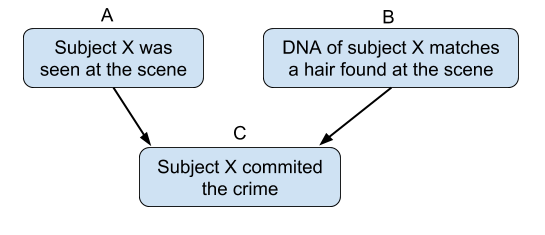
\includegraphics[width=0.9\textwidth]{img/Bayesian_Network}
\end{figure}
Each node holds a predicate, which is true with certain probability depending on the value of incoming nodes.
For example, a table of the node $C$ in the figure \ref{fig:bayesianNetwork} would describe conditional probabilities of the events $P(C | A, B)$ for all possible combinations of values A and B \cite{Vlek2016bayes}.
The \textit{Bayesian Network} enables to visualize the legal arguments and is able to work with uncertainty.
The probabilities of unlikely events are especially of great importance since judges need to distinguish between coincidence and purpose.

\section{Electronic Discovery}
Electronic Discovery, also known as E-discovery or Electronic Data Discovery (EDD), is a process of searching, gathering, cleansing, and organizing of legal documents in order to find evidence in a civil or criminal legal case \cite{Conrad2010ediscovery}.
The field of Information Retrieval (IR) is an essential part of the E-Discovery, as it provides efficient full-text search among the documents.
\citeauthor{Conrad2010ediscovery} mentions how the IR can be supplemented by AI techniques in his work \citetitle{Conrad2010ediscovery} \cite{Conrad2010ediscovery}:
\begin{enumerate}
\item Intelligent relevance feedback
\item E-mail management
\item Social network analysis
\item Data mining and machine learning techniques
\item Anticipatory E-Discovery
\end{enumerate}
The E-mail and Social network have become naturally a source of legal arguments with increasing amount of information stored in such media.
Anticipatory E-Discovery is a new practice of corporates to prepare for a possible legal hold on some of their products or intellectual property.

The fourth category includes mainly the clustering and categorization of documents to organize them into separate groups.
A research under \textit{Xerox Research Center Europe} introduced a machine learning classifier \textit{CategoriX}, which works with a fixed set of document categories and predicts document's category with probabilistic latent semantic analysis (PLSA) \cite{barnett2009classification}.
The mentioned technique is usually applied in the topic modeling of documents and is briefly explained in the section \ref{topic_modeling} as it is one of the working attributes of the system proposed here.
Research of Noortwijk et al. presents the \textit{Copac} system, which categorizes whole legal cases instead of documents.
Moreover, they relaxed the set of categories and enable users to define their own by selecting examples of positive and negative samples \cite{van2006ranking}.

The main goal of this research is the relevance prediction.
However, the categorization of documents is also part of this research, because the preparation for the relevance prediction is labeling documents as case-related or law-related (\ref{sec:law-case-classifier}).
The paper \citetitle{thompson2001automatic} compares three algorithms for legal document classification: k-NN, decision tree algorithm, and a machine learning rule induction algorithm Ripper \cite{thompson2001automatic}.
They conclude the decision tree and Ripper algorithms outperform the k-NN with Ripper being best by recall measure.
For the purpose of the categorization discussed in this research, a decision tree was applied for its satisfactory performance, simplicity, and transparentness.
Moreover, the ensemble of decision trees -- Random Forest -- helped us to boost the performance.

The first enhancement of IR -- Intelligent relevance feedback -- best explains the workflow of the system proposed here.
By feedback, \citeauthor{Conrad2010ediscovery} means consultation of the suggested relevance by the system to the user, which might lead to recomputation of the relevances \cite{Conrad2010ediscovery}.
This iterative process has proven to increase the accuracy of the predictions \cite{Conrad2010ediscovery}.
On the other hand, Zhao et al. show that more than one round of the feedback selection process is not helpful \cite{zhao2009feedback}.
The proposed system provides a possibility of immediate feedback through relevance settings of individual documents.
Relevances within the scope of the particular legal case are updated after each feedback.

To compare the existing systems with the proposed, it is worth noting that most of them implement a slightly different use case.
Their goal is to pick relevant documents out of a massive storage of legal texts, in which documents might relate to multiple cases, whereas here the goal is to pick relevant documents out of a relatively small collection that is uploaded to the system by the lawyer.
The proposed system is not allowed to share documents among cases nor look for information elsewhere than what is selected by the lawyer.
This task is somewhat more difficult since the prediction model starts to learn almost from the beginning with each new case.
Most of the similar researches focus either on the case retrieval or document retrieval from a global storage, hence the use case of the proposed system seems to be too unusual to be included in any recent research.

% Papers predicting outcomes of new cases based on previous
% 1. Automatically classifying case texts and predicting outcomes

\section{Measuring relevance in legal domain}
\label{sec:related_relevance}
Many studies are concerned with the concept of relevance in the legal domain, formalization of its subjective nature and its measuring and evaluation (\cite{vanOpijnen2017relevance}, \cite{Hogan2010sensemaking}, \cite{Ashley2010analysis}).
The following discussion takes into consideration a human ability to decide the relevance.

% paper: Document categorization in legal electronic discovery: computer classification vs. manual review.
When evaluating relevance decided by an automated system, the results should be always compared to the efficiency of humans.
Results in IR and E-Discovery are hard to evaluate since there is no ground truth.
Even among the humans annotators, the 100\% agreement is simply not possible -- the relevance is too subjective factor.
Roitblat et al. conduct an experiment that compares efficiency of computer classification and manual review \cite{roitblat2010comparison}.
They pick 5000 documents from a collection of 1.6 mil documents (9.8\% relevant) annotated by attorneys in the past for other purposes than research.
Consequently, a new group of attorneys divided into two teams A and B were reviewing the documents.
At the same time, two anonymous E-Discovery systems referred to as C and D were applied to classify all collection of 1.6 mil documents.
Precision of the manual reviews (percentage of correctly relevant from all classified as relevant) was 20\% and 18\% whereas the systems achieved precisions of 27\% and 29\%.
Recall of the manual reviews (percentage of correctly relevant from all relevant) was 49\% and 54\% whereas the systems achieved recalls of 46\% and 53\% \cite{roitblat2010comparison}.
Note that the the recalls are quite comparable, whereas the precision is significantly higher for the classification systems.
This research showed that the time invested in development of such systems is worthwhile.
The present research will refer to these results in the evaluation chapter (\ref{chp:evaluation}) to compare the precision and recall to both the human efficiency and state-of-the-art legal classification systems.

% Relevance - with higher precision, lower recall and vice versa, always better high recall
% paper: Automation of legal sensemaking in e-discovery
In ordinary IR, the precision is usually more significant measure than recall, since the user is often satisfied with the first few most relevant results.
In the legal domain, both high precision and high recall are required, sometimes the recall is considered the dominant measure as missing a relevant information could be fatal \cite{Hogan2010sensemaking}.
Hogan et al. divide the E-Discovery systems to two groups according to the method for balancing precision/recall.
First group is the CAHA systems (Computer Assisted Human Assessment), where humans assess and filter the result of the IR system \cite{Hogan2010sensemaking}.
The IR system returns a result with low precision but high recall and human selection rises the precision.
The other systems are HACA (Human Aided Computer Assessment), in which a human provides an annotated samples of documents to improve models of the IR system \cite{Hogan2010sensemaking}.
Here, the HACA system is a fully automatic system with high precision and high recall.
This research presents a system that falls into the latter group.

% paper: On the concept of relevance in legal information retrieval
Opijnen and Santos in their study \citetitle{vanOpijnen2017relevance} breaks down the relevance into six concepts, which are necessary to ensure relevant result \cite{vanOpijnen2017relevance}.
Whereas they understand the relevance in context of the IR, Hogat et al. in their study \citetitle{brassil2009usermodeling} relates the relevance to a supervised classification system, which is closer to the system presented here \cite{brassil2009usermodeling}.


As the definition of relevance is entirely derived from the user's requirements, Hogan et al. present a User Modeling (UM) approach to achieve high performance in search tasks \cite{brassil2009usermodeling}.
The four main concepts of UM are:
\begin{enumerate}
\item \textit{Use Case} -- determines the goals of the user and their preference towards precision and recall.
\item \textit{Scope} -- defines the relative amount of concepts that are understood by the user as relevant. The scope defines a threshold that tell which concepts are \textit{core} and which are \textit{peripheral}.
\item \textit{Nuance} -- is a measure determining how relevant are concepts within a document, considering lexical relationships.
\item \textit{Linguistic Variability} -- determines the variability of expressions of the concept. The expressions can be lexical or syntactic.
\end{enumerate}

% paper: Emerging AI & Law approaches to automating analysis and retrieval of electronically stored information in discovery proceedings

\chapter{Background: Legato System}
The system introduced in this research is integrated into a proprietary web application \textit{Legato} developed by the \textit{SDE Software Solutions Ltd.} company.
\textit{Legato} is a collaborative system for management of legal documents that provides comprehensive control over legal cases including full-text search, organizing of important information and visualizations.
The system is now in development phase undergoing a number of user testing in U.S. and Czech environment.

\begin{figure}[h]
\caption{Legato -- Dashboard}
\label{fig:legato_dashboard}
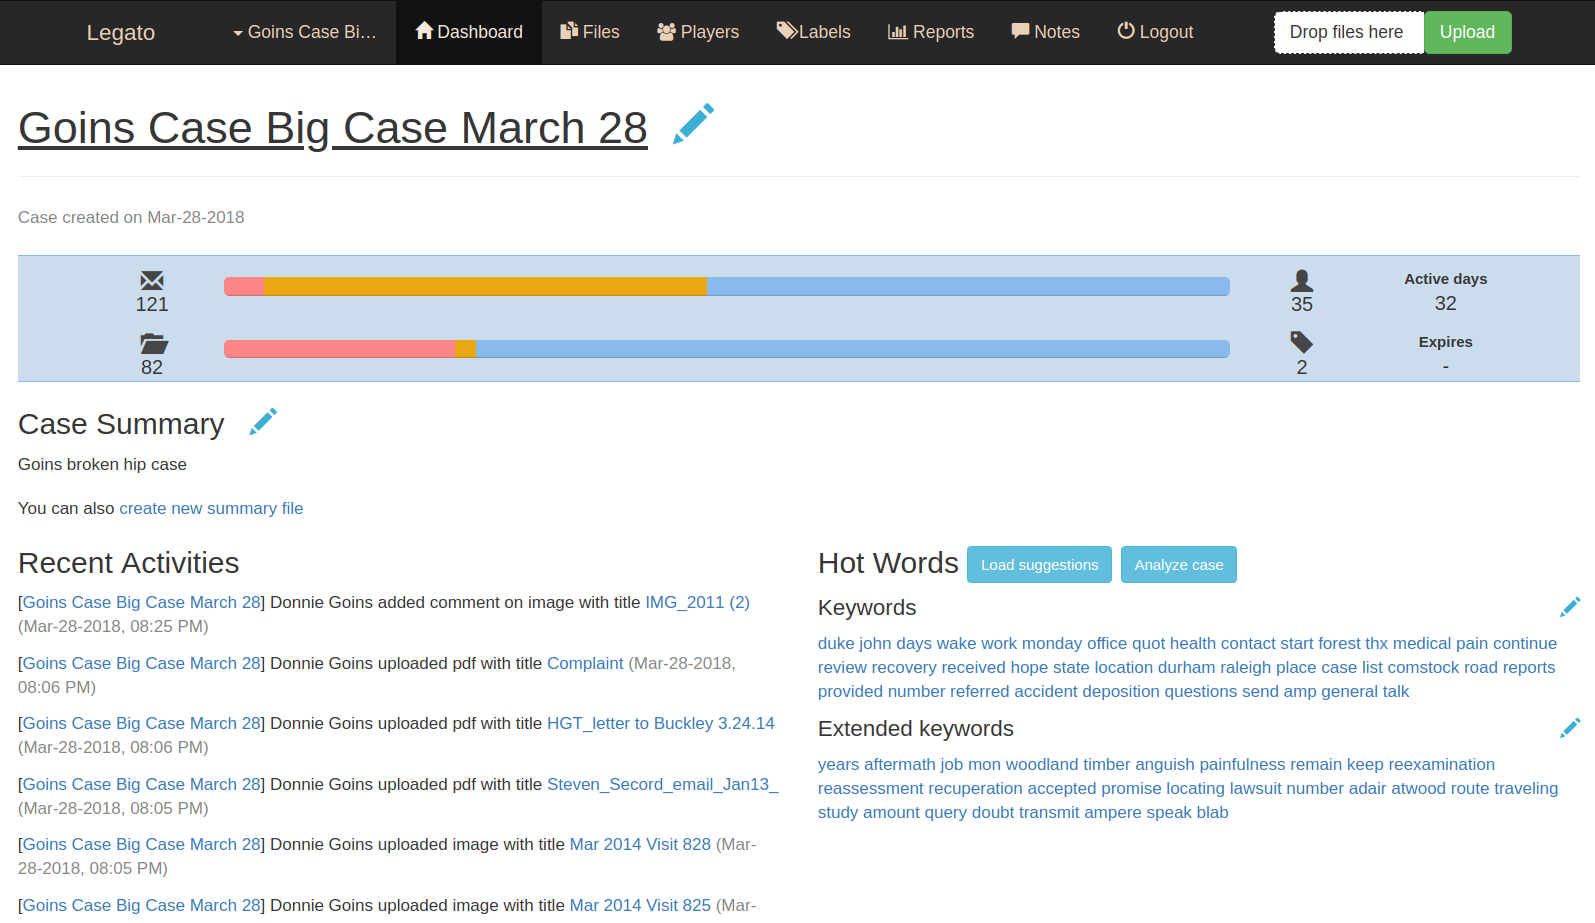
\includegraphics[width=\textwidth]{img/Legato-Dashboard}
\end{figure}


\section{Use case}
\label{sec:legato_usecase}
Legato belongs to the group of E-Discovery systems, which provide an infrastructure mainly to the lawyers and attorneys, who need to collect legal documents from both sides (plaintiff and defendant) and possibly from other sources, such as the World Wide Web.
The next phase of E-Discovery is the organization of documents and information retrieval tasks to find relevant pieces of information in the texts.
\textit{Legato} is designed to ease and speed up the E-Discovery in general.

Legato expects the following workflow of a paralegal working with the system.
Firstly, the user obtains data from various sources and loads them into Legato.
Subsequently, the user is able to skim through the documents to get high level overview of the case.
The user categorizes the documents according to the type and source (doctor reports, police reports, personal emails, agreements, etc).
Then, a rough prioritization takes place -- the user sees the most promising documents based on the entities recognized from the text.
In the next phase, the user goes through the promising documents, makes notes, extracts important information, keywords and players to understand the case in depth.
The last step is a report compilation, in which the user gathers collected notes and important documents to construct the most promising strategies for a defense or accusation.

Users can upload documents in various formats (plain text, PDF, image, etc.), which is followed by a phase of post-processing.
The document is converted into plain text or analyzed by the \textit{OCR} in case it is an image.
Then, it is analyzed by third-party libraries to extract additional features.
So far, there are only two types of documents: emails and others.
Emails are treated specially for their metadata and are further utilized to provide deeper insight into data (more in \ref{sec:legato_advanced}).

Figure \ref{fig:legato_dashboard} displays a home page of a legal case in the \textit{Legato}.
Here, the user is able to see various statistics about the case including a number of emails and other documents, number of document labels, number of players, number of days of active work on the case, recent case activity, case summary, overview of relevance and main keywords.

Labels serve users for annotation of documents by custom text tags.
Some users might label the origin of documents, others might distinguish confidential document from the public one and others might label simply their favorites.

The term \textit{player} is understood as a person, who appears and is directly involved in the case.
At the moment, \textit{Legato} has no tool to automatically recognize players from documents other than extracting sender and receiver from emails.
In the future, users will be able to add their own players and NLP tools will help to recognize them from the documents.

The figure \ref{fig:legato_document} shows a document detail page.
Besides reading, users can highlight arbitrary part of a document and add a commentary.
Thanks to the OCR analysis, the system is able to show a plain text version and enables text selection, full-text search, and copying.


\begin{figure}[h]
\caption{Legato -- Document}
\label{fig:legato_document}
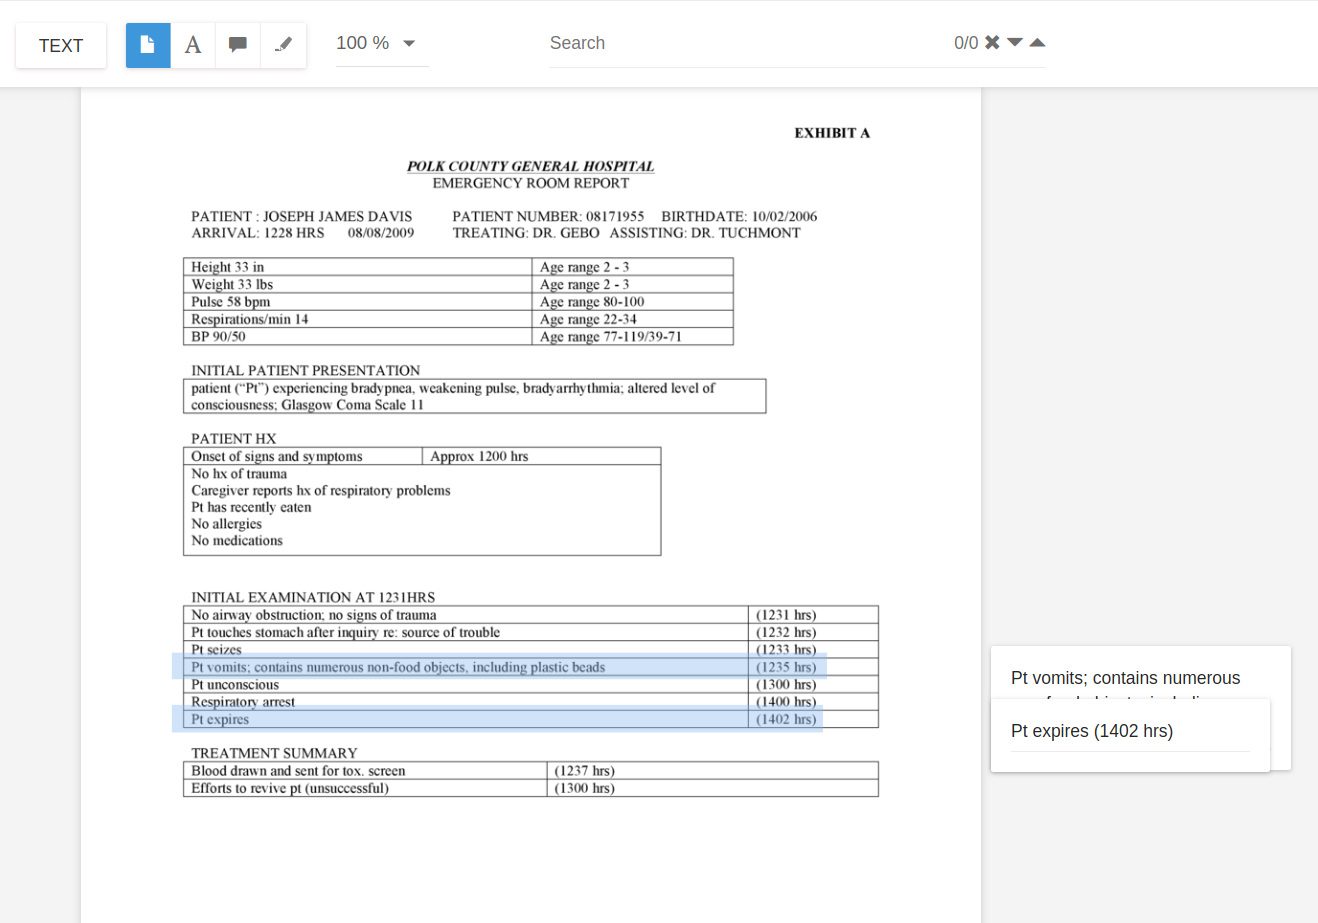
\includegraphics[width=\textwidth]{img/Legato-File}
\end{figure}

\section{Technical details}
The backend of Legato is written in PHP language using the \textit{Laravel}\footnote{PHP web framework \url{https://laravel.com}} web framework.
All application instances run on \textit{Debian}\footnote{Stable Linux operating system \url{https://www.debian.org/}} server in the \textit{Apache}\footnote{Web container \url{https://httpd.apache.org/}} container.
Legato stores all data into the \textit{PostgreSQL}\footnote{Open source relation SQL database \url{https://www.postgresql.org/}} database.
There are multiple instances of Legato, depending on their purpose: alpha is the production instance, demo serves for the user testing and ai is enriched with innovative features.
The \textit{Amazon Web Services}\footnote{Collection of cloud computing services \url{https://aws.amazon.com/}} ensures the infrastructure and enables deployment, monitoring and debugging services.

\section{Research \& Advanced Features}
\label{sec:legato_advanced}
Thanks to the progressive attitude of \textit{Legato} management, multiple advanced features were proposed.
The ideas of management and developers are often amazing features with a rich functionality; however, only some of them intersect with the user's requirement, which explains the excessive user testing.

\subsection*{Natural Language Processing}
One of the most important features is the recognition of named entities in the text (more in the section \ref{sec:named_entities}).
Named entities, such as people, companies, locations or dates are key pieces of text that lawyers might look for.
As management of \textit{Legato} is aware of that, they are intensively researching the most suitable tool for named entity extraction together with other natural language processing (NLP) features.
One of the most wanted features is the \textit{text summarization}, which could accelerate the process of reading and sorting of documents.
Unfortunately, the \textit{text summarization} is too abstract and still very hard task for automated NLP systems to be competitive with humans.

% Email reconstruction and timeline
\subsection*{Email reconstruction}
One of the features that are already implemented, is the email reconstruction and timeline.
Emails contain enough structured metadata for the full reconstruction of conversations including senders, receivers, subjects and dates (fig. \ref{fig:legato_email}).

\begin{figure}[h]
\caption{Legato -- Email}
\label{fig:legato_email}
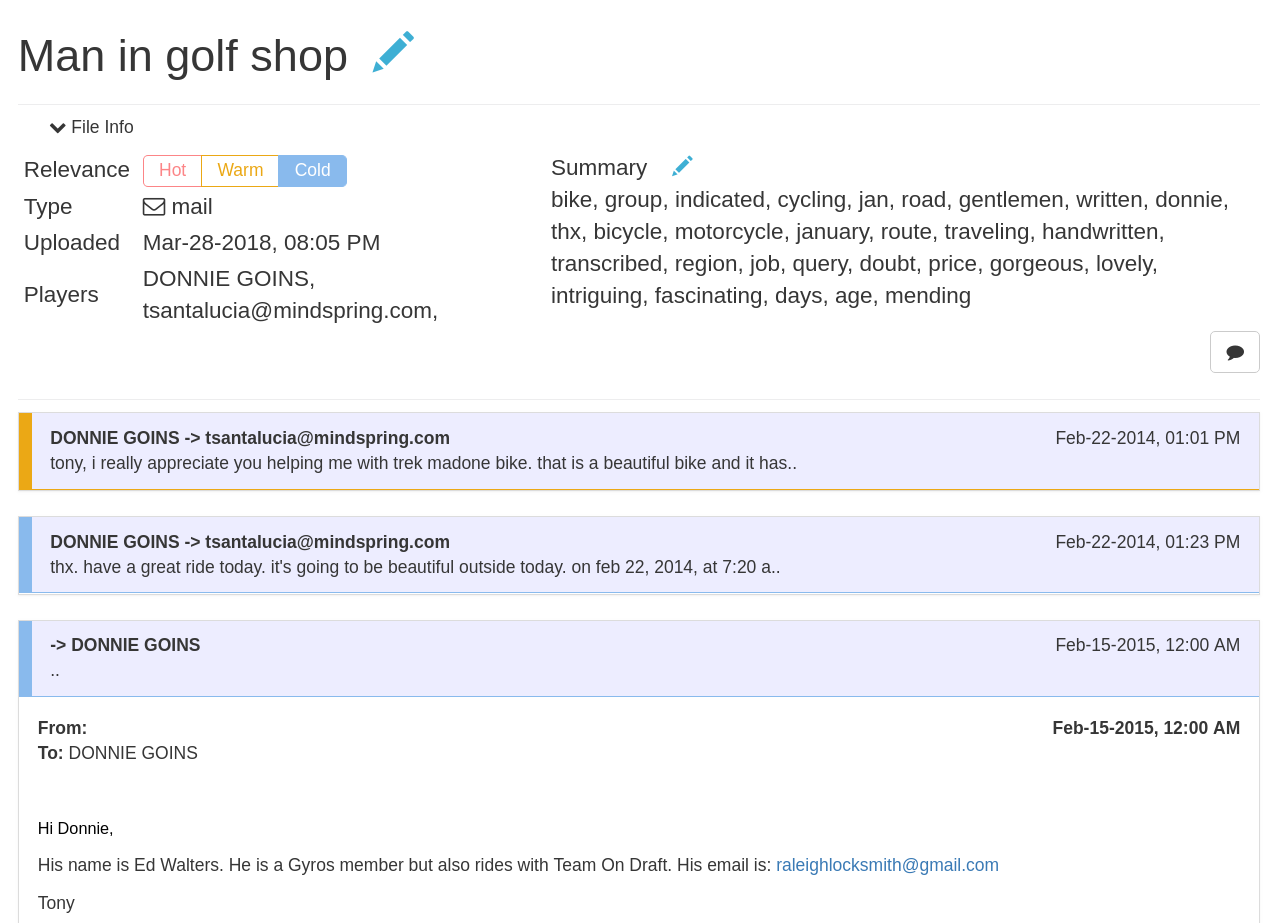
\includegraphics[width=\textwidth]{img/Legato-Email}
\end{figure}

\subsection*{Timeline}
Dates are also applied in the timeline visualization (fig. \ref{fig:legato_timeline}), which consists of points representing emails horizontally arranged by date.
The color of points marks the relevance and the size represents the number of emails in the conversation.
When a conversation stretches across multiple days, the points are connected by a line.

\begin{figure}[h]
\caption{Legato -- Timeline}
\label{fig:legato_timeline}
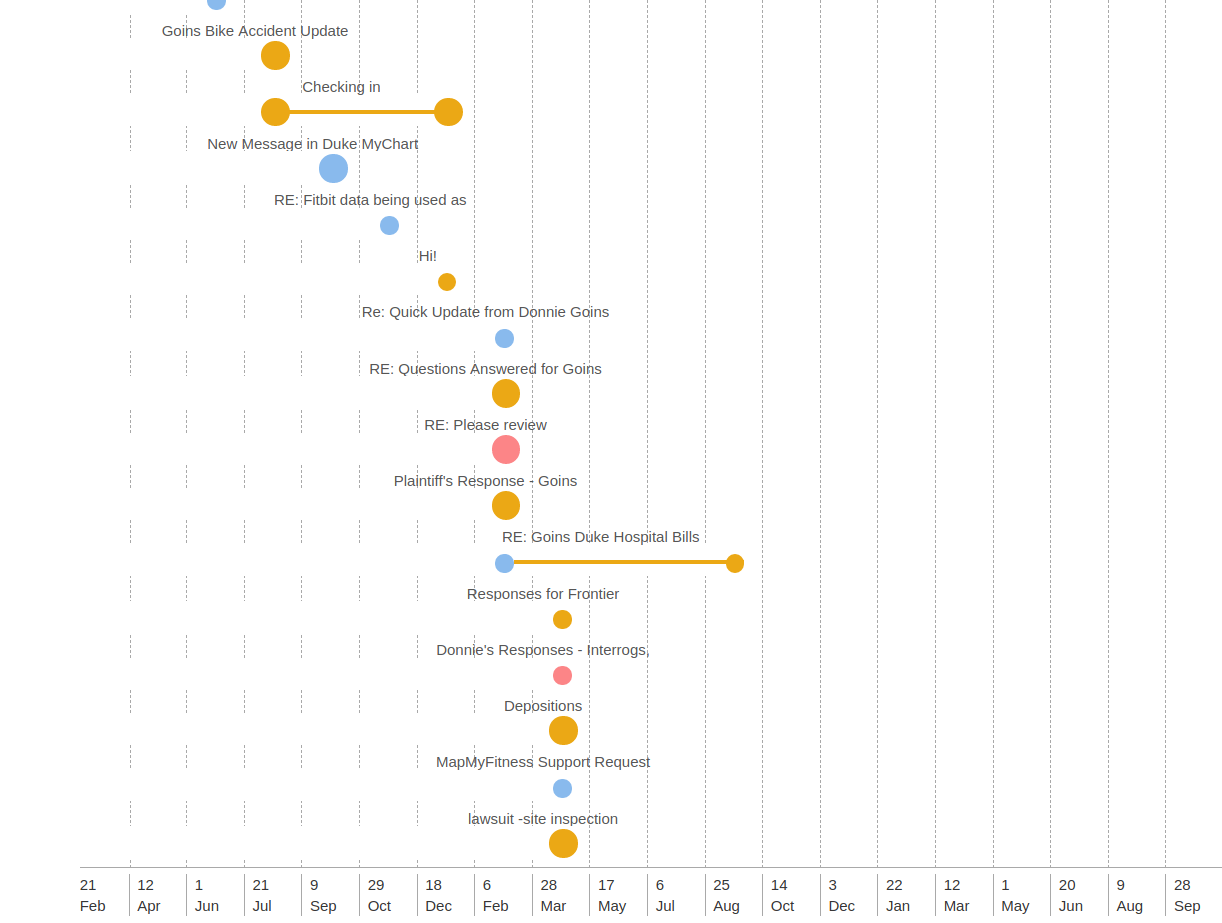
\includegraphics[width=\textwidth]{img/Legato-Timeline}
\end{figure}

\subsection*{Communication chart}
Due to quite reliable identification of the players in the communication, it is possible to draw a circular communication chart (fig. \ref{fig:legato_communication}).
Players' names are printed into a circular shape and two players are connected if and only if there exists an email that was sent from one to the other.

\begin{figure}[h]
\caption{Legato -- Communication chart}
\label{fig:legato_communication}
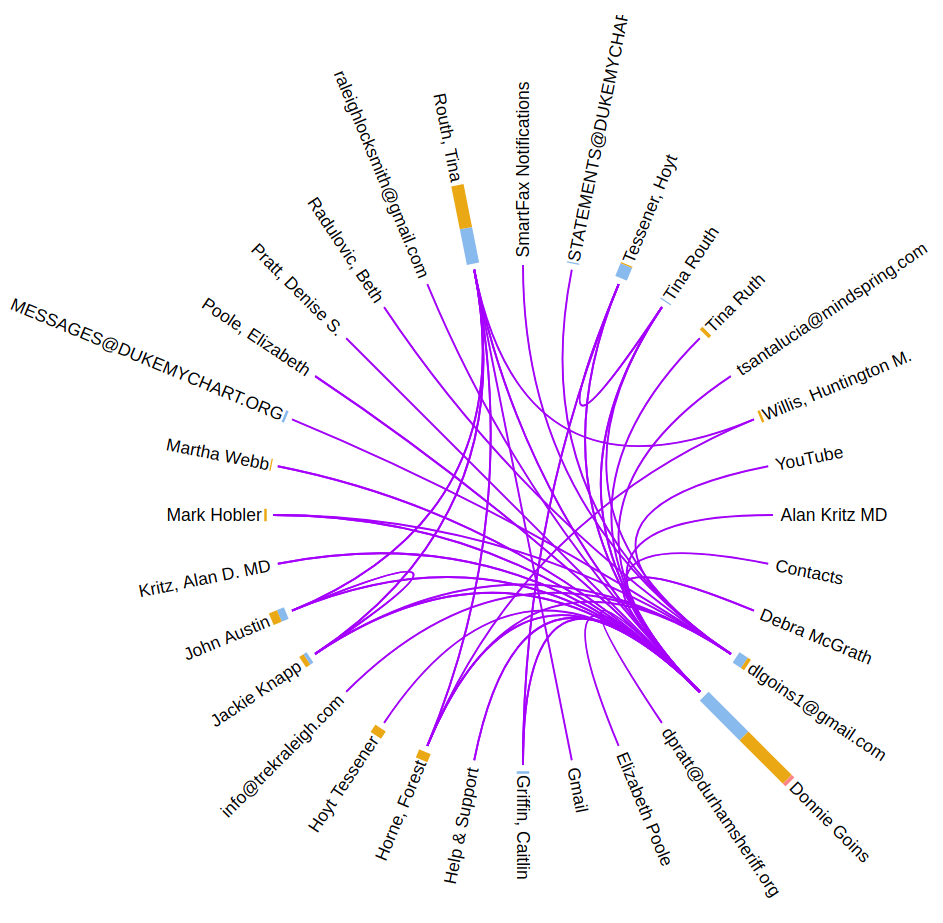
\includegraphics[width=\textwidth]{img/Legato-Communication}
\end{figure}

\subsection*{Annotation of images}
Another already implemented feature is the image annotator.
Whenever an image is uploaded into \textit{Legato}, Google Vision API \footnote{\url{https://cloud.google.com/vision/}} automatically recognized concepts in the picture and creates tags.
This feature helps with structuralization of data and adds images into results of full-text searches.

\subsection*{Optical Character Recognition}
An \textit{Optical Character Recognition} (OCR) is the very essential part of every E-Discovery system.
Although some documents are already in the electronic form, such as emails or PDF document, lawyers have to work with a large number of only-paper documents too, that needs to be scanned.
OCR is then applied to the scanned documents to extract text in the electronic form.
Even though there has been a wide investment in the algorithms for OCR, the result is never 100\% successful because the recognition leaves some "typos".
The better algorithms use some statistical models to guess the most probable word.

Research in \textit{Legato} team about the best OCR tool is still ongoing and the performance of this step is taken very seriously, as the result influences the outcome of all subsequent steps of the E-Discovery. The tool used at the moment is called \textit{Tesseract}\footnote{\url{https://github.com/tesseract-ocr/tesseract/wiki}}, which is one of the open source projects focused on OCR.



\chapter{Data Characteristics}
\label{chp:data_characteristics}
One of the most important preconditions for building an efficient model is to understand the input data characteristics.
People developed numerous models based on text classification that are suppose to classify text of any domain, however, at the expense of the efficiency.
The specialized models always have the potential to outperform the general one.
The real contribution of this work is the understanding of characteristics of the legal domain data and its application on the process of building a text classification model.
This chapter will introduce our working dataset, its statistics and characteristics.

\section{Dataset introduction}
The end users of the Legato system are mostly the U.S. lawyers, which influences our choice of the dataset.
The U.S. legal system is very specific with its own laws, constitution, trial process and most importantly for us -- terminology.
Also, we have to take into consideration specifics in the form of the documents: medical records, police records, affidavits, emergency call transcripts etc.
We do not claim that our application will not work for other than U.S. legal documents, however, the model might manage to recognize the structure and terminology of the U.S. documents more accurately.

Unfortunately, we have not acquired enough training data from the users of Legato, mainly because the legal cases are ongoing and the documents are too confidential to be included in a research.
For the same reason, it is hard to find an authentic public trial documents on the Internet.
We have found a solution thanks to an \textit{American Mock Trial Association} \footnote{http://www.collegemocktrial.org/} and \textit{Classroom Law Project} \footnote{\url{http://www.classroomlaw.org}}.
Both associations create legal cases for educational purposes, which then serve as a material for the mock trial competitions.
All their legal cases are fictional, though some of them were inspired by real-world situations and issues.
Still, any resemblance to actual persons and events is purely coincidental.

All 20 cases used as a training set are downloaded from two sites: Street Law, inc. \footnote{\url{http://streetlaw.org}} and Classroom Law Project \footnote{\url{http://www.classroomlaw.org}}.
Not to be biased with one legal area, we included cases of diverse legal fields:
\begin{itemize}
\itemsep0em
\item[2x] \textbf{School environment} \\ educational malpractice or indifference
\item[1x] \textbf{Bullying} \\ intentional infliction of emotional distress
\item[2x] \textbf{Criminal law} \\ assault, battery or murder
\item[3x] \textbf{Inmate partner violence} \\ domestic violence by a current or former partner
\item[3x] \textbf{First Amendment} \\ breach of freedom of speech, religion, press etc.
\item[4x] \textbf{Child neglect} \\ child injury or death caused by parents, baby-sitter or teacher
\item[2x] \textbf{Sex crime} \\ sexual harassment and disease transmissions
\item[3x] \textbf{Tort law } \\ fault leading to suffer or harm, without breaching any contract
\end{itemize}
All mock cases have a similar structure: there are approx. 5-8 testimonies of the involved people, called affidavits, and the rest of the documents are emails, medical records, police reports, emergency call transcripts, description of the past similar cases etc.
The affidavits are up to 10 pages long, usually describing the issue in depth, whereas the other documents are usually one or two pages long.
We excluded all extra information specific to the mock trials, explanations of the competitions and summaries: we do not expect these to be typical part of a case.
Some extra headers and footers that contain metadata were also removed not to confuse the model training.

During the model building, we need to take into account that the real cases might be more or less different from the mock cases.
For instance, we do not expect the affidavits to appear in the real cases as much as in the mock cases.
Also, we expect more emails and papers of unknown structure in real cases.
Generally, we found two major shifts: 
\begin{enumerate}
\item real cases will most probably contain shorter documents
\item real cases will contain many more unrelated documents
\end{enumerate}
We present solutions for both issues:
\begin{enumerate}
\item 
The length of the document should be an insignificant parameter when determining the documents relevancy.
Therefore, we decided to focus on sentences rather than on a document as a whole.
In other words, we determine relevance of the document by exploring the relevances of the individual sentences.
As a result, the model is slightly simplified, however, we do not completely ignore the cross-sentence information, as we will see in the further chapters.
Thanks to the sentence-based model, we should be able to eliminate an influence of the document length and judge the relevance without bias.

\item
The second issue is caused by the lack of motivation to add unrelated documents during the creation of the mock cases.
Still, we can find some documents that are related to the case but are not relevant, e.g. resume of a defendant.
A straight forward solution is to add some irrelevant documents from other cases to simulate the balance in a real situation.

\end{enumerate}

\section{Annotation}
- num of annotators
- annotation of docs
- annotation of sentences

\section{Data statistics}
As mentioned earlier, we are working with 20 cases with total of 261 documents, which means 13.15 documents per case in average.
The documents together contain 234,798 words, thus average number of words per document is 900.
We counted 14,518 unique words which is approx. 1.18 \% of English vocabulary according to the \textit{Oxford English Dictionary}  \cite{oxfordDictionaries}.

\begin{figure}[h]
\centering
\caption{Most frequent words in the dataset with and without stop words.}
\label{fig:most_frequent}
\footnotesize
\begin{tabular}{|l|r||l|r|}\hline
\rowcolor{orange!50}
\multicolumn{2}{|c||}{\makebox[9em]{\textbf{All words}}} & \multicolumn{2}{|c|}{\textbf{Without stop words}} \\\hline\hline
\textbf{word} & \textbf{count} & \textbf{word} & \textbf{count} \\\hline\hline
the & 10825 & school & 855 \\\hline
to & 6632 & would & 683 \\\hline
I & 6274 & one & 566 \\\hline
and & 5912 & time & 497 \\\hline
of & 5479 & 1 & 476 \\\hline
a & 4896 & said & 451 \\\hline
in & 3603 & told & 420 \\\hline
that & 3499 & could & 409 \\\hline
was & 2846 & get & 391 \\\hline
for & 1942 & like & 386 \\\hline
\end{tabular}
\normalsize
\end{figure}

In the left part of the figure \ref{fig:most_frequent}, we present counts of the most frequent words in the documents.
It is not a surprise that all top ten words are common stop words of English.
The stop words are usually removed before any further processing of the text, however, they might carry valuable information too.
For instance, recognition of the author or formality level can be determined based on the stop words usage.
We can see that the usage of stop words is not different from the general English.

The right side of the table shows most frequent words after we removed the stop words.
Here, we can see clear influence of the cases from the school environment.
Next, the words "said" and "told" indicate that the documents often contain reporting of events and conversations.
The other words again fit more or less in the general English.

The word frequencies tell us that the vocabulary is not biased by any major trend.
Lets now look at the keywords of the whole collection and discover words that occur more frequently than usual.
The method used is explained in section \ref{algorithms_keywords} and we applied the same reference corpus (Reuters articles).
The following are the keywords: city, school, know, got, joey, just, police, princess, time, person, really, like, child.

- most frequent words for crime vs. first amendment
- most frequent words for relevant vs. unrelevant cases

\section{Types of documents}
- non-sense docs (pics)
- law related vs. case specific - loosely define
\section{Linguistics}


\chapter{NLP tool selection}
The amount of text in legal documents can vary largely.
Most of the documents we are working with stretch across one page, however, the average number of pages is six and we can find documents up to hundred pages long.
The typical approach of the text processing is to convert the text into a document-term matrix that contains number of term occurrences in each document.
The problem with this approach is that the long documents are represented by a vector, which \emph{information gain} is rather low.
High \emph{information gain} implies that the numerical representation captures the general idea, the purpose of the document, and characteristics of similarity/dissimilarity with other documents.

To address the issue, we decided to represent a document with specific features extracted by one or more NLP tools rather than plain words of the document.
We are looking for the most interesting pieces of information in the text, such as people, locations, dates, crime-related words or email addresses.
Nowadays, one can find numerous services providing extraction of such features.
We have chosen some of them and have collected results from testing on our mock legal case.
We compared results of the NLP services and a survey, in which participants labeled features from the text in a similar way as an NLP tool.

It is important to note that the field of NLP feature extraction is a well-studied topic and the tools produce very stable results, probably using rather similar algorithms (which are described in the following section). Even though we could dedicate part of this work to developing well-suited algorithms for NLP feature extraction, we decided to take advantage of the existing tools and put the focus on processing and application of the features to the high-quality data mining and machine learning algorithms. 

\section{NLP Algorithms}
First, let us introduce the features and well-known algorithms for their extraction from a text in general.
Note that the further mentioned tools might use modified or even different techniques for extraction of the features.

\subsection{Keywords}
\label{algorithms_keywords}
\emph{Keywords} are people, places, words, ideas, which are understood as important in the given context. 
In our case, the context is the document, hence we expect the keyword to reflect what the document is really about.
Then, the \textit{keyness} is a quality measure of the importance in the given text.
\cite[ch. 4]{scott2006textual}

We do not restrict the keyword to be one word because most of the tools are able to extract multi-word keywords, so-called \textit{key phrases}.
By combining words together, the phrases usually gain a new meaning that cannot be inferred from the individual words.
Therefore, if we assumed only one-word keywords, we would never find the keyness hidden in the phrases.

The process of identifying keywords is driven by two factors.
First, the more often a word occurs in the document, the more likely it is a keyword.
And second, the more often a word occurs generally in a speech, the less likely it is a keyword of any document.
\cite[ch. 4]{scott2006textual}
The second factor ensures that words we use very often in the speech, such as prepositions, conjunctions or the most common nouns, are not considered as keywords, even though their occurrence is frequent.

Common implementation of the idea is called the \textit{TF-IDF} algorithm \cite[ch. 6]{manning2008introduction}.
The weight of a term is defined by its \textit{term frequency} and \textit{inverse document frequency}.
The term frequency tf$_{t,d}$ is simply a number of occurrences of the term $t$ in the document $d$. The \textit{inverse document frequency} is defined as
$$
\text{idf}_t = \log{\frac{N}{\text{df}_t}}
$$
where $N$ is the total number of documents and df$_{t}$ is a \textit{document frequency}, which is equal to the number of documents containing term $t$.
It is important to take a logarithm of the expression because the \textit{inverted document frequency} can become very large with a large collection of documents and we need it to be comparable with the \textit{term frequency}, which is rather small.

The tf-idf weight is computed as follows \cite[ch. 6]{manning2008introduction}:
$$
\text{tf-idf}_{t, d} = \text{tf}_{t,d} \times \text{idf}_t
$$
The \textit{term frequency} ensures higher weight for more frequent terms in the document and \textit{inverse document frequency} ensures higher weight for more obscure words. Now, tf-idf$_{t, d}$ can be a good approximation of our keyness measure and is often used in the keyword extraction technique with the same same. The last step is to establish a threshold value that distinguishes keywords and non-keywords by comparing it to the tf-idf values of the terms.

\subsection{Named Entity Recognition}
\label{sec:named_entities}
To extract valuable information from the text, it is necessary to include \textit{named entities} (NEs).
They are entities that can be referred to with a proper name \cite[ch. 21]{jurafsky2014speech}.
In the speech, NEs are always noun phrases representing people, places, things, organizations, temporal or numerical expressions, events etc.

Lets pinpoint how important the named entities are in the context of legal cases.
Consider a typical use case of our application: a lawyer is searching through hundreds of emails with different senders and receivers.
The name of the only victim, place, and date of the crime are known.
If the lawyer is forced to manually search through the documents, they will filter the emails by occurrences of the aforementioned facts in the text.
All of the facts are named entities, which can be extracted from each document automatically and eventually lead the algorithm to increase the relevance of documents accordingly.
Thanks to the named entities, the algorithm performs the classification in the same manner as the lawyer would do, which is our goal.

The academic approach to find a \textit{named entity} is often based on the statistical sequence model \cite[ch. 21]{jurafsky2014speech}.
Entity type and boundaries are found with one pass over the text according to a set of rules.
The rules include \textit{Part-of-Speech Tagging} 
\footnote{Detailed information about POS Tagging can be found in chapter 10 of \citetitle{jurafsky2014speech} by \citeauthor{jurafsky2014speech} \cite{jurafsky2014speech}}
, which helps to find the noun phrases, and therefore, the boundaries.
Next, the \textit{word shapes} are examined, which are simple string representations that generalize a group of expressions.
For instance, replacing any letter for X and any digit for d, we can describe a unique word shape dd XX, which represents hours of the day written in US format, such as 12 am or 03 PM. 
Other rules include prefix matching or dictionary of predefined named entities.

In comparison to the academic approach, the commercial approach is based on the combination of updated dictionaries, rules and supervised machine learning \cite{chiticariu2013rule}.
In the word of Big Data, it has become easier to collect large dictionaries of given names, family names, organizations or geological places (gazetteers).
The named entity recognition is performed by multiple passes over the text data.
First, the high-precision but low-recall rules are applied, then more entities are added by substring search of the previous entities.
In the next phase, the entities are consulted with the dictionaries and only then, the statistical sequence model is applied considering all the features from the previous stages \cite[ch. 21]{jurafsky2014speech}.

Further in the thesis and the application, we will work with the following set of \textit{named entities}:
\begin{itemize}
\item Person
\item Organization
\item Location
\item Time
\item Email Address
\item Crime
\item Health Condition
\end{itemize}

\subsection{Relations}
Once we have extracted the \textit{named entities}, we can start looking for the relationships between them.
As soon as we recognize entities and their relations, the main semantic meaning of a sentence is usually fully extracted.
In the legal environment, we can illustrate the added value of a relation by a testimony, in which a witness tells about both a person and a location, however, we are interested in the document only if there is a relation between these two.

Lets see how the relations are represented.
Most of the \textit{relations extraction} algorithms are focused on binary relations only.
Multi-entity relations would be very expensive to extract.
We will borrow the representation from the Resource Description Framework (RDF) \cite{lassila1999resource} and define the relation as a triple
$$
\text{<subject, predicate, object>}
$$
where the \textit{subject} is an entity that performs an activity specified in the \textit{predicate} with respect to the \textit{object}.
In our context, the \textit{predicate} is the type of the relation; it can be, for example, "employed-by", "built", "son-of" or "cheated-on".

The following groups of algorithms can be applied to extract the relations: \textbf{hand-written patterns}, \textbf{supervised machine learning}, \textbf{semi-supervised}, and \textbf{unsupervised}.
We will introduce the first two
\footnote{For more detailed description, see \citetitle{jurafsky2014speech} \cite{jurafsky2014speech}.}.

\subsubsection{\textbf{Hand-written patterns}}
The work \citetitle{hearst1992automatic} by \citeauthor{hearst1992automatic} \cite{hearst1992automatic} describes the first idea of using patterns to extract relations.
The entity names are ignored and a relation is recognized by a set of patterns.
The patterns are based on the lexicology (POS tagging), the syntax (syntax tree) and the type of the entity (person, location, etc.).
For example, the pattern \cite[sec. 21.2]{jurafsky2014speech}
$$
NP_0\text{ such as }NP_1 \{, NP_2 ..., (\text{and|or})NP_i \}, i \geq 1
$$
is able to catch the relation hyponym for many occurrences, for instance, a sentence
$$
\text{... by any poison, such as Cyanide, Arsenic or Ricin ...}
$$
would generate relations 
\begin{itemize}
\item <poison, hyponym of, Cyanide>
\item <poison, hyponym of, Arsenic>
\item <poison, hyponym of, Ricin>
\end{itemize}
An example of a pattern using entity type \cite[sec. 21.2]{jurafsky2014speech}
$$
\text{\textbf{PERSON} (named|appointed|chose|...) \textbf{PERSON} Prep? \textbf{POSITION}}
$$
will determine a relation "named". 

The big disadvantage of the pattern-based recognition is that the patterns need to be written by hand, which takes a lot of work. On the other hand, the precision of such method is usually high since the patterns are directed by a human.

\subsubsection{\textbf{Supervised machine learning}}
The second approach is to annotate a corpus of relations and entities and consider it as a training set in the machine learning.
More precisely, features are extracted from the sentences and are served to the machine learning algorithm as an input.
With the relation types as the output labels, the algorithm is prepared to be trained automatically.
\cite[sec 21.2]{jurafsky2014speech}.

The features can consist of unigrams or bigrams of the words in the sentence, especially between the subject and object. Next, the named entity types, POS tags or features from the syntax tree can be included as well. Sometimes the number of words between the subject and object or stemmed version of the words is also be considered \cite[sec. 21.2]{jurafsky2014speech}.

The algorithm uses two models for the relations extraction.
The first decides whether there exists a relation between two given entities, and the second one recognizes its type. First, the algorithm finds all pairs of entities in the sentence, test it with the first model, and only the positive results are tested on type with the second model \cite[sec. 21.2]{jurafsky2014speech}.

The supervised method has a potential to be very accurate on general inputs, however, to achieve a better results than pattern-based models, a large training dataset is required.
Therefore, the \textit{Distant Supervision for Relation Extraction} was invented to solve the problem \cite{mintz2009distant}.
It is an elegant way, how to obtain a large training dataset.
The DBpedia \footnote{Comprehensive database of structured facts extracted from Wikipedia: \mbox{\url{http://wiki.dbpedia.org/}}} or 
Google Knowledge Graph \footnote{Database of world knowledge structured in a graph: \url{https://www.google.com/intl/bn/insidesearch/features/search/knowledge.html}}
provide enough information about some of the relations between real-world objects.
The algorithm is able to extract full relations with subject, object and relation type.
To gather the training data, the algorithm searches a page about the subject on Wikipedia and finds a sentence with the specified object.
Then, it is ready to adopt the text as an input data for the training phase.
This approach delivers a lot of diverse sentences, in which we are confident about the relation type, and thus the training dataset is rich enough to create a reliable model.

\subsection{Topic Modeling}
\label{topic_modeling}
The \textit{Topic modeling} is a statistical approach for finding general topics that appear in the document.
The keywords are already able to discover some trends of a document, however, unlike the topics, they have to appear in the text.

Prior to the topic recognition, a fixed set of topics have to be defined.
The more advanced algorithms creates a hierarchical topic structure rather than a simple list.
The usual process of topic modeling is to assign probabilities of all topics to every word in the dictionary.
Then, if we consider a document as a bag-of-words
\footnote{Representation of a document that forgets ordering and counts of the words and keeps them in a simple set.}, 
we can compute the overall probability that a document has a specific topic only from its words.

One of the well-known algorithms for the topic modeling is called the \textit{Latent Dirichlet allocation} developed by \citeauthor{blei2003latent} in \citeyear{blei2003latent} \cite{blei2003latent}.
The model assumes that every document has a fixed distribution of topics it belongs to.
Let's further assume that the words of a document were withdrawn from a specific distribution defined in the following way.
\begin{enumerate}
\item Pick a topic distribution of each document according to a \textit{Dirichlet distribution}.
\item Pick a word distribution for each topic.
\item For all words in all documents, generate the word as follows:
\begin{enumerate}
  \item Pick a random topic according to the distribution of topics for the document.
  \item Pick a random word from the distribution of words for the topic chosen in the step a).
\end{enumerate}
\end{enumerate}
The generation scheme tells us the probability theory for documents and topics, however, it does not tell us how to recognize the topics from the fixed documents.
To apply the theory, we need to reverse the process and assume that the documents were created by this generation process, and eventually guess the topic.
One of the iterative methods, which achieves this goal, is called the \textit{Collapsed Gibbs Sampling} \cite{xiao2010efficient}.
Put simply, the initialization phase picks a random topic for each word in all documents and each next phase goes over every word and changes its topic by computing the probabilities, assuming that all the other words are correctly labeled.



\subsection{Document Category}
There are two types of categories we are interested in.
The first is more related to the structure of the text and tells us where the document is coming from. 
Such types can be for instance email, medical record, police record, affidavit, etc.
The Legato system is prepared to work with such categories, and therefore, we rely on the input to contain the information about the first type.

The second type is related to the meaning of the text.
Semantically, it is very similar to the topics introduced in the section \ref{topic_modeling}, and the only difference is that we need the most dominant topic to be chosen as a representative.

\section{Introduction of the tools}

\subsection{NLTK: The Natural Language Toolkit}
As a baseline for the commercial NLP tools, we included the open source python framework \textit{NLTK} \cite{bird2004nltk}.
Although it was originally developed for educational purposes, it is now broadly used by students, researchers and public to process the textual data in python.

\textit{NLTK} consists of multiple modules, which can be used as a pipeline during the text processing. 
The basic modules run the tokenizer, POS tagging, and syntactic analysis.
More advanced modules are dealing with the information extraction and knowledge representation.
The framework comes with large preprocessed corpora that can be used as reference corpora during the keyword or NE extraction \cite{bird2009natural}.

The commercial NLP tools do not need any settings since they are already configured and the configuration is basically the key to their success.
Nevertheless, the \textit{NLTK} is more a framework than a tool and we have to take the time to set the variables right.
It also brings a great advantage of highly configurable settings.
In the next two paragraphs, we explain our approach to extracting the keywords and entities in the \textit{NLTK}.

We applied the \textit{TF-IDF} algorithm to compute the keywords, as explained in \ref{algorithms_keywords}.
Firstly, we removed the stop words and filtered only meaningful words.
The list of stop words was used as defined by the \textit{Scikit-learn library} \footnote{Machine learning library for python \cite{pedregosa2011scikit}}.
To remove the nonsense words, we compared them against a dictionary of the \textit{Brown corpus}, which is the first text corpus of American English of about 1 million words \cite{brownCorpus}.
Next, we filtered only nouns and finally, computed the \textit{TF-IDF} score against the \textit{Reuters} reference corpus \cite[sec. 2.1]{bird2009natural}, which contains more than 10,000 news articles with 1.3 million words.
We have chosen the journalistic context because it was the closest domain to the legal environment.
This procedure outputs a score for each word in a document and the final keywords are those, which \textit{TF-IDF} score was more than a threshold of 0.15.

The entity extraction requires fewer settings since the NE tagger is already trained by the library \cite[sec. 7.5]{bird2009natural}.
We split the text into sentences and consequently sentences into tokens \footnote{token = word as a string without a disambiguated meaning}.
Next step is to extract the part-of-speech tags for each token.
The tokens together with the \textit{POS tags} are the input data into the \textit{NE chunker}, which is able to mark words as named entities and also determine its type.


\subsection{Google Cloud Natural Language}
Google has a long-standing experience with the text processing, especially in the field of information retrieval.
They decided to provide their knowledge of semantic text analysis in a service called Cloud Natural Language \cite{googleNLP}.
Google makes no secret of their approach: the same Deep Learning models that power the Google Search are also employed in the NLP service.

The tool is able to recognize entities, syntactic structure of sentences, category and sentiment of the text.
The sentiment analysis is recently very interesting topic because companies want to know public opinion of themselves.
However, the sentiment in legal documents is usually neutral and does not play a key role in the relevance classification, therefore we decided not to consider sentiment as a feature.

The \textit{Cloud Natural Language} tool also adds a level of confidence to every entity and category so that the user see how strong each feature is. Moreover, the tool replies with a Wikipedia article for every entity, if exists. Another useful feature is the Translation API, which converts text among many different languages and is able to recognize sources of an unknown language. Worth noting that the input does not have to be a pure text but also speech in the audio format or text in a picture.

\subsection{Watson Natural Language Understanding}
In March 2017, the IBM announced retirement of the \textit{AlchemyAPI} service, which was designed to understand the semantics of text and image by advanced techniques \cite{alchemyRetirement}.
One component of the service was also the \textit{AlchemyLanguage}, providing all NLP features, such as entity, sentiment and topic recognition.
As a replacement, a new service emerged: the \textit{Natural Language Understanding} service \cite{watsonNLP}.

Besides typical NLP features, such as keywords, entities, relations, category, sentiment or topics (which are called concepts in the \textit{NLU}), the service provides emotion recognition (joy, anger, fear, etc.) and metadata recognition.
The latter includes basic information about the author, title, prominent page image, and publication date.
Unfortunately, this feature is available only for HTML pages, which is usually not the type of our documents, hence we will not take advantage of the metadata recognition.

One of the most promising features of the \textit{NLU} service is the model customization.
All the NLP features are always recognized with respect to some general language model, which consists of words from all aspects and domains of our language.
This might be a disadvantage, especially when our documents are actually always of one type and contains words from a specific domain.
For instance, the general model would always consider law, justice or  sentence as keywords in our legal documents, however, they might appear in most of the documents and become not relevant anymore in the legal domain.
The \textit{NLU} service enables a user to create its own language model and load it into the cloud.
More than one model can be active and the user can switch between them before each query.

\subsection{Aylien}
\textit{Aylien} is a software package of information retrieval, machine learning, and natural language processing \cite{aylienNLP}, which provides competitive features to the mentioned NLP services from Google and IBM.

In addition to the classical NLP features, \textit{Aylien} provides summarization, which essentially picks the most important sentences from the text. In fact, this feature makes a good sense in our legal domain. Next innovative feature looks for related phrases, which are semantically as close to the original phrase as possible. Another advantage of \textit{Aylien} is that it includes time-based entities in the named entity recognition, specifically, dates. The previously mentioned services surprisingly ignore the time and date expressions most of the time.

Next interesting feature of \textit{Aylien} is the hashtag suggestion, however, it is basically the topic modeling as we described it in \ref{topic_modeling}.
In the same manner, the article extraction is another term for the IBMs metadata recognition.
Truly new feature is the aspect-based sentiment analysis, in which the sentiment is recognized for each aspect, not generally for the whole text.
For example, an analysis of hotel reviews can discover angry opinions on Wi-Fi signal but an excellent rating of the staff.

\section{Comparison}
To compare the tools, we had to restrict the evaluation set only to the common features included in all the tools.
Specifically, the \textit{keywords} and \textit{named entities}: persons, organizations, and locations.
Without any comparison, we also evaluated the relations, which were supported only by \textit{Watson NLU}, and dates supported only by \textit{Aylien}.

\subsection{Testing data: Legal mock case}
Of course, we could not use any real-world case for our testing and analysis due to privacy reasons, therefore, we analyzed a legal mock case called \textit{Davis v. HappyLand Toy Company}\cite{american2015davis} created by the \textit{American Mock Trial Association}\footnote{http://www.collegemocktrial.org/}.

Briefly described, the case puts a father of a child, who was killed by swallowed part of a toy, against the company that produced the dangerous toy. For our use case, we picked five most interesting and distinct documents: 
\begin{enumerate}
\item An email of an inter-company communication about the substances used in the toy.
\item Affidavit (testimony) of the father.
\item Affidavit of the babysitter, who looked after the child at the moment of the fatality.
\item Medical record from the autopsy of the child.
\item Journal paper about the origin, behavior, look, and impacts on a human body of the substance used in the toy.
\end{enumerate}

\subsection{Survey}
The survey was created in a way that no knowledge of the law is necessary, the questions are simple and clearly stated.
Some of the documents are several pages long, hence the survey can be saved and finished later.
The respondents were not provided with any extra information about the legal case so that the results are comparable with the NLP tools, which have no information as well.
The survey was completed by five developers of the Legato system.

We asked the same set of questions for every document.
First two questions asked about the keywords.
We have split the one-word phrases and multi-word phrases and required both with at least 10 one-word keywords.
Next, the respondent has to type people, organizations, and locations that appear in the text.
Moreover, we require relationships between people and dates together with a label specifying which event is related to the date.
Next two questions were related to the semantics and were not used to evaluate the tools.
We asked the respondents to copy a short passage from the text that could be used as an evidence at the court.
The second question asks for a short summary of the whole document.
Both of the questions will be later applied in the training and evaluation of the models
for document relevancy.


\subsection{Statistical comparison}
\label{sec:nlp:statistical_comparison}
\begin{figure}
\centering
\caption{Jaccard index of the NLP tools evaluated against the survey with strict string comparison.}
\label{fig:jaccard_table_strict}
\footnotesize
\begin{tabular}{|l||l||*{5}{c|}}\hline
\rowcolor{gray!30}
\makebox[4em]{\textbf{Feature}}&\backslashbox{\textbf{Document}}{\textbf{Tool}}
&\makebox[3em]{\textbf{NLTK}}&\makebox[3em]{\textbf{Google}}
&\makebox[3em]{\textbf{Watson}}&\makebox[3em]{\textbf{Aylien}}\\\hline\hline
Keywords & Miller affidavit &0.11&&0.11&0.02\\\hline
& Davis affidavit &0.06&&0.03&0.03\\\hline
& Email &0.05&&0.24&0.20\\\hline
& Toxicology paper &0.00&&0.02&0.03\\\hline
& Medical record &0.09&&0.04&0.05\\\hline\hline
& \textbf{Average} &\textbf{0.06}&&\textbf{0.09}&\textbf{0.07} \\\hline\hline
People & Miller affidavit &0.00&0.29&0.54&0.38\\\hline
& Davis affidavit &0.00&0.13&0.25&0.24\\\hline
& Email &0.29&0.44&1.00&0.43\\\hline
& Toxicology paper &0.00&0.00&0.29&0.00\\\hline
& Medical record &0.00&0.27&0.71&0.57\\\hline\hline
& \textbf{Average} &\textbf{0.06}&\textbf{0.23}&\textbf{0.56}&\textbf{0.32}\\\hline\hline
Organizations & Miller affidavit &0.07&0.40&0.50&0.29\\\hline
& Davis affidavit &0.06&0.17&0.33&0.17\\\hline
& Email &0.00&0.25&0.50&0.00\\\hline
& Toxicology paper &0.00&0.33&0.33&0.14\\\hline
& Medical record &0.00&0.00&0.00&0.00\\\hline\hline
& \textbf{Average} &\textbf{0.03}&\textbf{0.23}&\textbf{0.33}&\textbf{0.12}\\\hline\hline
Locations & Miller affidavit &0.00&0.06&0.00&0.00\\\hline
& Davis affidavit &0.00&0.00&0.00&0.00\\\hline
& Email &0.00&0.00&0.00&0.00\\\hline
& Toxicology paper &0.00&0.00&0.00&0.00\\\hline
& Medical record &0.14&0.00&0.00&0.00\\\hline\hline
& \textbf{Average} &\textbf{0.03}&\textbf{0.01}&\textbf{0.00}&\textbf{0.00}\\\hline\hline
\end{tabular}
\normalsize
\end{figure}

\begin{figure}
\centering
\caption{Jaccard index of the NLP tools evaluated against the survey with subset tolerance in string comparison.}
\label{fig:jaccard_table_subset}
\footnotesize
\begin{tabular}{|l||l||*{5}{c|}}\hline
\rowcolor{gray!30}
\makebox[4em]{\textbf{Feature}}&\backslashbox{\textbf{Document}}{\textbf{Tool}}
&\makebox[3em]{\textbf{NLTK}}&\makebox[3em]{\textbf{Google}}
&\makebox[3em]{\textbf{Watson}}&\makebox[3em]{\textbf{Aylien}}\\\hline\hline
Keywords & Miller affidavit &0.30&&0.47&0.57\\\hline
& Davis affidavit &0.35&&0.26&0.33\\\hline
& Email &0.14&&0.57&0.50\\\hline
& Toxicology paper &0.09&&0.37&0.25\\\hline
& Medical record &0.23&&0.24&0.15\\\hline\hline
& \textbf{Average} &\textbf{0.22}&&\textbf{0.38}&\textbf{0.36} \\\hline\hline
People & Miller affidavit &0.79&0.32&0.85&0.94\\\hline
& Davis affidavit &0.64&0.29&0.63&0.47\\\hline
& Email &1.00&0.56&1.00&0.71\\\hline
& Toxicology paper &0.00&0.06&0.29&0.29\\\hline
& Medical record &0.57&0.40&0.71&0.83\\\hline\hline
& \textbf{Average} &\textbf{0.60}&\textbf{0.32}&\textbf{0.69}&\textbf{0.65}\\\hline\hline
Organizations & Miller affidavit &0.36&0.40&0.50&0.71\\\hline
& Davis affidavit &0.06&0.17&0.33&0.17\\\hline
& Email &0.50&0.50&1.00&0.50\\\hline
& Toxicology paper &0.29&0.33&0.33&0.29\\\hline
& Medical record &0.16&0.00&0.00&0.00\\\hline\hline
& \textbf{Average} &\textbf{0.27}&\textbf{0.28}&\textbf{0.43}&\textbf{0.33}\\\hline\hline
Locations & Miller affidavit &0.27&0.61&0.67&0.29\\\hline
& Davis affidavit &0.00&0.10&0.00&0.00\\\hline
& Email &0.00&0.00&0.00&0.00\\\hline
& Toxicology paper &0.00&0.00&0.00&0.00\\\hline
& Medical record &0.14&0.00&0.00&0.00\\\hline\hline
& \textbf{Average} &\textbf{0.08}&\textbf{0.14}&\textbf{0.13}&\textbf{0.06}\\\hline\hline
\end{tabular}
\normalsize
\end{figure}

Since the survey was completed by only five respondents, we decided to unify results for each answer.
The standard approach how to compute agreement between two sources is the \textit{Cohens kappa measure} \cite{smeeton1985kappa}.
The problem with \textit{kappa measure} is that the sources assign a fixed number of items to classes, which is not our situation.
In our case, the number of items is variable and we do not have any classes.
We care about the agreement between the sets.
Therefore, we are using a measure for the distance between sets, the \textit{Jaccard index} \cite{levandowsky1971distance}, defined as follows:
$$
J(A, B) = \frac{|A \cap B|}{|A \cup B|}
$$
Since the union is always larger than or equal to the intersection, we get $0 \leq J(A, B) \leq 1$ for any sets $A$, $B$. 
When $J(A,B)=1$, the sets are identical and when $J(A,B)=0$, the sets do not share any item.

The next step is to define when two items (keywords and entities) are equal.
We have defined two approaches in comparing the equality: \textit{strict approach}, and \textit{subset tolerance approach}.

In the \textit{strict approach}, all items are converted to lower case, so that the names, organizations, locations and other items are compared regardless of the capital letters.
Apart from that, no changes are made to the items and the comparison is based on a strict string equality.
As a consequence, for instance, full name and given name alone are not equal, even if the text represents the same person. 
E.g. for sets $A=\{\text{"Joey Davis", "Brett"}\}$ and $B=\{\text{"Joey", "Brett"}\}$ the Jaccard index is 
$$
J(A, B) = \frac{|\{\text{"Brett"}\}|}{|\{\text{"Joey Davis", "Joey", "Brett"}\}|} = 1/3
$$
Figure \ref{fig:jaccard_table_strict} shows \textit{Jaccard indices} using the strict approach for each combination of tool, feature and document compared with the ground truth, which is the survey output.
The "\textbf{Average}" row displays the mean over all documents for each tool and feature.

The \textit{subset tolerance approach} converts the items to lower case in the same manner as the \textit{strict approach}.
Then, two items are equal if one is a subset of the other or they are strictly equal.
To keep the construction of unions and intersections simple, we include both superset and subset in the union as well as in the intersection.
E.g. for sets $A=\{\text{"Joey Davis", "Brett"}\}$ and $B=\{\text{"Joey", "Davis"}\}$ the Jaccard index is 
$$
J(A, B) = \frac{|\{\text{"Joey Davis", "Joey", "Davis"}\}|}{|\{\text{"Joey Davis", "Joey", "Brett", "Davis"}\}|} = 3/4
$$
Results of the \textit{subset tolerance approach} are displayed in the figure \ref{fig:jaccard_table_subset} in the same form as in \ref{fig:jaccard_table_strict}.
One can notice that the score is always equal or higher compared to the \textit{strict approach}, which is a natural consequence of the approach definitions.

\subsubsection{\textbf{Keywords}}
All tools except for the \textit{Google Cloud Natural Language} service provide the keywords extraction.
The \textit{Jaccard index} is generally very low in the case of the keywords.
There is usually a lot of words to choose from and even the respondents agreed only on few of them.
We can notice the best scores in the case of the email due to the short length of the text.
The \textit{Watson NLU} achieved the best score, however, it did not perform much better than our baseline \textit{NLTK}.
\textit{Aylien} scores high in the \textit{subset tolerance approach} because it extracts very long keywords, which have a high probability of being superset of some of the real keyword.

\subsubsection{\textbf{People}}
The scores for the people extraction were surprisingly high.
In the \textit{strict approach}, the \textit{NLTK} failed because of its limitation of recognizing only one-word items.
People names mostly appeared with both given and family name and the \textit{NLTK} recognized the name separately as two items.
On the other hand, when the subsets are tolerated, the \textit{NLTK} achieved very good result.
The winner of this category is the \textit{Watson NLU}, which is superior for every document and approach.
\textit{Aylien} service achieved a better score than \textit{Google CNL}, especially in the case of the longer documents.

\subsubsection{\textbf{Organizations}}
The \textit{NLTK} achieved the lowest score for the same reason as in the case of the people extraction since the names of organizations also consist of more than one word.
In the strict variant, all other tools performed significantly better than the baseline, yet the best score again achieved the \textit{Watson NLU} service.
In this category, \textit{Google CNL} outperformed the \textit{Aylien} service in the \textit{strict approach}, however, we can see reversed result in the \textit{subset tolerance approach}.
One of the possible explanations is the fact that \textit{Google} is able to precisely determine borders of the entities but they are not so often common with the survey output.
Whereas \textit{Aylien} usually fails at determining the borders since the organizations often consist of many words but the items contain the right information in the subsets.
The Medical record, unfortunately, does not contain many organizations, therefore none services were successful.

\subsubsection{\textbf{Locations}}
The extraction of the locations was quite chaotic and diverse by the respondents as well as by the tools.
The location can be understood as a named entity which is unique in the world, such as Hype park in London, 107 Myers street or Moscow, whereas someone understands the location as any expression specifying the environment, such as living room, school or a car.
The latter type was mostly recognized by the \textit{Google CNL} and the other tools recognized the first type.
Moreover, there were not enough location entities in the documents to draw a meaningful conclusion from the results.
In the strict variant, we ascribe win of the \textit{NLTK} service to a coincidence, as its simple model extracted many words starting with capitals, hence more people than locations appeared in the output set.
In the subset tolerance variant, \textit{Google CNL} and \textit{Watson NLU} achieved very similar score, however, the Watson generated approximately ten times fewer items, which brings us to a conclusion that the discriminative power of the Watsons items might be higher.

\subsubsection{\textbf{Dates}}
As the \textit{Aylien} service is the only one that is able to extract the time-based entities, we have not performed any comparison.
Still, we wanted to see how precise is the extraction, and so we present the \textit{Jaccard index} computed from the \textit{Aylien} output and the survey data.

\begin{figure}[h]
\centering
\caption{Jaccard index of the time-based entities extracted by Aylien.}
\label{fig:jaccard_dates}
\begin{tabular}{|l||*{5}{c|}}\hline
\rowcolor{gray!30}
\makebox[4em]{\textbf{Document}}&{\textbf{Jaccard index}}\\\hline\hline
Millers affidavit & 0.07 \\\hline
Davis affidavit &0.13\\\hline
Email &0.00\\\hline
Toxicology paper &0.00\\\hline
Medical record &0.00\\\hline\hline
\textbf{Average} &\textbf{0.04}\\\hline
\end{tabular}
\end{figure}
The \textit{Aylien} achieved non-zero results only in the longer documents and even then, the scores are under our estimation.
As an example, a simple date in form "24. 12. 2017" is recognized as a phone rather than a date.
Here, it strongly depends on the spaces: after we remove a space before the month -- "24.12. 2017" -- the day and month are finally recognized as a date, however, the whole string is still reported as a phone.
On the other hand, we took into consideration only the dates, while \textit{Aylien} recognizes times and other expressions, such as "last week", as well.

\subsection{Analytical comparison}
Aside from the statistical evaluation of the tools accuracy, it is also important to manually analyze the output and check whether it is semantically correct.
In this section, we discuss characteristics of the tools and their benefits and drawbacks.

\subsubsection{\textbf{NLTK}}
We already outlined two drawbacks of the \textit{NLTK} in the previous section: one-word limitation and simple NE model.
The first problem is visible in both affidavits, where the toy name appears under the name "Princess Beads", which is an obvious keyword in this context.
Interestingly, the \textit{NLTK} extracted both parts: "princess" and "beads" as keywords since the words are quite unique by itself.
However, the key phrase was missed.
As the \textit{NLTK} is highly customizable, we believe that the multi-word phrases extraction is indeed possible but it would require an extra amount of work.

On the other hand, the keyword extraction performance was very well comparable to the commercial tools.
\textit{NLTK} performed considerably worse in the entity extraction.
Besides the separation of the given and family name, it also falsely marked "Liquid", "Myth" or "Identification" as people, probably because of the capital letters.
One can notice a lot of false positives in the Medical record, were a lot of words were written in the capitals and \textit{NLTK} recognized all of them as organizations, e.g. "BODY", "AND" or "OF".

Although the \textit{NLTK} provides a very good baseline for the NLP feature extraction, we can see a noticeable line between its hand-written patterns and the supervised machine learning models, which are used by the other tools.

\subsubsection{\textbf{Google Cloud Natural Language}}
The approach of the Google is a little different in the following way.
Together with the entity, it outputs also a position in the text and it does not discard duplicates.
\textit{Google} does not understand the extraction as picking of the most identifying words, but more as a highlighting of the words in the text.
Therefore, the \textit{Google CNL} usually produces a larger output than others.
The true positive rate is almost perfect, for example in the Millers affidavit, all of "Brett Miller", "Lee Davis", "Andy Davis", "Hillary Davis" and "Joey Davis" were recognized.
Even more surprising is that "Hillary Davis" appears only once in the text and \textit{Google} was able to link the name to many occurrences of her given name.
The problem is that words, such as "kids", "one", or "friend" are recognized as well, and truth is that they really represent some people in the meaning, however, it is not necessary and rather disturbing in our use case.

\subsubsection{\textbf{Watson Natural Language Understanding}}
The \textit{Watson} approach is slightly more moderate.
Very little false positives are introduced as \textit{Watson} outputs a word only in case of high confidence.
Similarly as \textit{Google}, \textit{Watson} recognized all people in the Millers affidavit including full name of "Hillary Davis".
Due to the conservativeness, only the family name of "Chase Tuchmont" was recognized since "chase" is an ordinary word in English as well.
However, the overwhelming majority of the recognized entities makes perfect sense and are truly people, organizations or locations.
Therefore, the \textit{Watson NLU} service is not only superior in the statistical evaluation, but also in the analytical overview of the semantics.

\subsubsection{\textbf{Aylien}}
We can see yet another approach by the \textit{Aylien} service.
Keywords are understood as complex pieces of information of arbitrary length, sometimes even more than 10 words long.
As a result, service correctly extracted "Joye" as a keyword in the Davis affidavit, though incorrectly extracted a key phrase "Davis and that I wanted to speak with someone about Princess", which seems rather awkward.
This was a source of a low score of \textit{Aylien} in the keywords category.

On the other hand, \textit{Aylien} excelled in the extraction of people.
Again, all people in the Millers affidavit were successfully recognized, even though the model was not sophisticated enough to merge "Hillary" and "Hillary Davis".
Despite a few mistakes, mostly recognizing numbers as people, the service was able to keep high true positives and low false positives, including organizations and locations.


\chapter{Classification}
Data exploration in the chapter \ref{chp:data_characteristics} helped us clarify the language and style of the legal documents enough to design models for the relevance classification.
% ... write about the outcomes of data characteristics chapter when they're done ...

First section (\ref{sec:attributes}) presents how the NLP features are encoded into attributes applicable to the models.
Next sections describe the system of models that predicts the document relevance.
Due to a large number of features, the system is structured into layers, where the top-level models make predictions based on the outputs of the bottom-level models.
The section \ref{sec:bottom-level-models} introduces the bottom-level models, which are specialized on each feature separately and are able to understand the word embeddings.
The top-level layer is formed by a pipeline of three machine learning models that are consecutively making decisions about the documents to output the final relevance.
First is the \textit{Law-Case classifier} \ref{sec:law-case-classifier}, second is the \textit{Sentence classifier} \ref{sec:sentence-classifier} and the last is the \textit{Document classifier} \ref{sec:document-classifier}.
Each of them needs a different set of inputs and applies different machine learning model.
The following figure visually explains the system of models.
For further details about the individual classifiers, see the related sections.

% TODO write that there'll be a lot of claims proven in evaluation section

\begin{figure}[H]
\caption{Diagram of models}
\label{fig:models-diagram}
TBA
\end{figure}

\section{Attributes}
\label{sec:attributes}
To achieve a successful classification, one of the most crucial steps is to convert the data into suitable attributes that will be most helpful in determining the classes.
Technically, all machine learning models are built to process numbers as input variables.
Since we work here with the text only, we have to find a way how to convert all keywords, entities, relations, syntactic structure, and other features into the numerical representation.
During this process, one has to keep in mind the main purpose: the numbers must internally hide information about the relevance.

Based on the arguments made in the chapter \ref{chp:data_characteristics}, the units of the machine learning are sentences rather than documents.
As a result, there is fewer data from which to compute the attributes and the representation of the attributes as well as the process of classification itself become simpler.

\subsection{Text preprocessing}
The extraction of features by NLP services and extraction of structural characteristics (sec. \ref{sec:structural_characteristics}) needs to be applied on the original raw text.
However, for the purpose of the sentence meaning extraction (sec. \ref{sec:sentence-meaning}), the first step is a text preprocessing.

The documents come into the Legato system in one of the two formats: a text in a digital form or an image.
The latter needs to be converted into the former, which is achieved by the Optical Character Recognition (OCR).
Unfortunately, the OCR technique is not perfect and leaves specific artifacts in the text.
Therefore, we first apply the text processing, which filters, edits and removes these artifacts and prepares the text to be segmented into sentences.

Firstly, all empty lines are removed and consecutive white spaces are converted into a single space character.
Secondly, the OCR artifacts has to be removed.
For example, the recognition puts '\&\#39;' instead of the apostrophe and '\&quot;' instead of the quotation.
Another artifact of the OCR are coupled words with missing spaces -- a dictionary of English words is applied to break the words apart.
Next, the text is converted into lowercase and filtered to keep only the alphanumerical characters.
The final step is a removal of a hyphenation that was introduced to break new lines in the original document.

\subsection{Sentence meaning embedding}
\label{sec:sentence-meaning}
When extracting a meaning of a sentence, one will encounter two major problems to be solved: 1) how to represent the meaning of a single word 2) how to combine word meanings.

The first problem is also known as the \textit{Word Embedding} problem \cite{wordEmbeddings}.
The simplest solution is to assign unique numbers to all words and train classifiers on the numbers instead of words.
$$
\{\text{"knife"} \rightarrow 1, \text{"gun"} \rightarrow 2, \text{"wire"} \rightarrow 3, \dots\}
$$
This approach does not usually perform well since the classifiers interpret a number as a quantitative, not nominative,  attribute.
As a result, the classifier understands two words with close numbers as close by the meaning as well.
Since the numbers were assigned without any order, there is undoubtedly a lot of misinterpretation.

The next solution is often applied in the information retrieval systems.
Instead of one number, we can represent the word embedding by a vector, with all elements zeroed but one.
Each word is assigned an unique index, on which the vector keeps a value of one.
$$
\{\text{"knife"} \rightarrow (1,0,0,0), \text{"gun"} \rightarrow (0,1,0,0), \text{"wire"} \rightarrow (0,0,1,0), \dots\}
$$
Now, a vector uniquely identifies a word and the vectors are not quantitatively comparable, which eliminates the problem with the previous approach.
This solution can be further improved by counting the words in the training documents, TF-IDF weighting or co-occurrence matrices \cite{wordEmbeddings}.

The third and final solution goes further in the embedding of semantics.
Recent research by Mikolov et al. \cite{mikolov2013efficient} introduced a revolutionary algorithm \textit{Word2vec}, which uses a neural network to create a vector of fixed length with its semantics compressed.
Each dimension of a vector represents some concept, which can be somehow quantified, such as masculinity, age or liveliness \cite{mikolov2013linguistic}.
The vectors are capturing semantic regularities, and therefore, the classifiers have a potential to perform better even for unknown words.
This embedding satisfies our ultimate assumption that close vectors are also close by the meaning of their underlying words.

Both the algorithm and the trained vectors are publicly available.
Though we could use the algorithm to train our own vectors, it is much easier to adopt the already trained dataset.
Since the meaning of the words is the same regardless of the area, there would be a very little gain in the training of a custom dataset specialized on legal documents.
The dictionary adopted here is trained by the \textit{Google} company and is available in their official code archive \cite{word2vecGoogle}.
The pre-trained model contains 3 million unique words of 300-dimensional vectors, which was trained on a 300 billion word news dataset.
For our purpose, a trimmed dataset of 300 thousand unique words without the phrases is sufficient \footnote{Downloaded from \url{https://github.com/eyaler/word2vec-slim}}.

The second problem relates to the fact, that the classifiers usually need fixed input, but the computed vectors exist for each word of a sentence.
Researchers Vedantam et al. \cite{vedantam2015learning} applied a simple average of \textit{word2vec} vectors to the words in a phrase to get the final embedding.
The idea can be extended to whole sentences by computing an average of all words in the sentence.
To achieve more interesting results, it is possible to weight the words by their TF-IDF score in the overall average, however, the contribution is not necessarily positive since the ordinary words can distinguish relevant sentence as well as the keyword.
Besides, the keywords (words with high TF-IDF) are embedded in another representation introduced in the next section, hence the TF-IDF weighting does not bring enough contribution to be worth the processing time.

\subsection{Keyword embedding}
Next attribute is a vector computed from the keywords that appear in a sentence.
The NLP feature extraction determined keywords in the context of the whole documents, which means the first task is to find the working set by intersecting the sentence with the keywords.
In the process of intersecting, the \textit{subset tolerance approach} is applied, as defined in the section \ref{sec:nlp:statistical_comparison}.

The next step is very similar to the approach mentioned in the previous section -- the words are converted into an embedding by the \textit{word2vec} dictionary and then averaged into one 300 dimensional vector.
Indeed, the sentence meaning vectors contain the keywords as well, thus some information is redundant and one can argue that these two attributes appear too similar.
However, the choice of right words plays a crucial role in the influence on classification, and the importance of both the attributes will be justified in the evaluation chapter.

\subsection{Entity embedding}
\textit{Watson NLU} service is able to recognize extensive number of entity types (462) \footnote{\url{https://console.bluemix.net/docs/services/natural-language-understanding/entity-types-v1.html\#entity-types-and-subtypes-version-1-}}, 
which include as obscure categories as "WebBrowserExtension" or "HockeyConference".
For the purpose of this research, only 6 of them the following types are used:
\begin{itemize}
\item Person
\item Organization
\item Location
\item Crime
\item HealthCondition
\end{itemize}
Note that also "Company" type is recognized, subsequently classified as "Organization".
In addition, the concepts and dates are included as entities, since there is no difference in the way they might influence the relevance.

The first draft of the entities embedding was based only on the entities appearing in the case.
During the case preprocessing, the mentioned entities were extracted from the case synopsis and stored in a vector of fixed length for each entity type. For instance, a vector for people entities might look as follows:
$$
(\text{"joey david", "thomas", "jesse hester", "obama", "", "", "", "", "", ""})
$$
The rest of the vector is left for entities from documents, which would be included based on their importance score (\textit{Watson NLU} attaches the score to each entity).
Finally, the representation is a mask array of ones and zeros that indicates which entities are present in the sentence.

One problem with this embedding is that the vector acquires different meaning for every case.
In a situation when a model learns that a name on the index $i$ indicates a relevant document, the model becomes not transferable to another case, where the vector contains different names.
General model for any case would become impossible to train and even the case-specific models would face a lack of data to achieve a satisfactory performance.
Fortunately, the \textit{word2vec} dictionary was trained on general texts including the entities as well.
Most of the well-known names, such as "David", "George", or "Adele", organizations, such as "Mc Donald", "IBM", or "Facebook" and locations, such as "Prague", "Nigeria", or "Prater" are present in the dictionary.
Not only that we can now train a general model, in which each word has its own fixed representation, but also the embeddings satisfy the expected semantic rules.
For example, vectors representing names will be close together and the model has a chance to learn that names are in fact important regardless of the specific word.


\begin{figure}[H]
\centering
\caption{Distances among entity vectors in word2vec dictionary.}
\label{fig:entity_distances}
\begin{tabular}{|*{5}{c|}}
  \hline
           & David   & George  & IBM      & Facebook \\ \hline
  David    & 0.0     &         &          &     \\ \hline
  George   & 0.93944 & 0.0     &          &     \\ \hline
  IBM      & 1.37978 & 1.41457 & 0.0      &     \\ \hline
  Facebook & 1.37652 & 1.40856 & 1.319643 & 0.0 \\ \hline
\end{tabular}
\end{figure}

TBA - explain the table and make conclusion

\subsection{Relation embedding}
\label{sec:relation_embedding}
The relations computed by Watson NLU keep the following structure:
\begin{listing}[H]
\begin{minted}[frame=single,
               framesep=3mm,
               linenos=true,
               xleftmargin=21pt,
               tabsize=4]{js}
{    
 "type" : "locatedAt",
 "sentence" : "her coming into the courtroom late"
 "arguments" : [
    { "text" : "her", 
      "entities" : [{ 
      	"text" : "her", 
      	"type" : "Person" }] 
    }, 
    { "text" : "courtroom",  
      "entities" : [{ 
      	"text" : "courtroom", 
      	"type" : "Facility" }] 
    }], 
}
\end{minted}
\caption{Watson NLU relation example in JSON} 
\label{json:relation}
\end{listing}
Note that the fields "location" and "score" were excluded to make the example compact.
As the JSON example suggests, the important parts of the relation are its type ("locatedAt"), types of the entities ("Person", "Facility") and the text of the entities ("her", "courtroom").
The relation embedding, therefore, needs to accommodate relation type, 2x entity type and 2x entities itself.
The previous sections presented the \textit{word2vec} dictionary, which is able to convert common words into a vector.
The same approach is used here for embedding of the entity words since there is a high probability of them being in the dictionary.

On the other hand, types of relations and entities are rather identifiers than meaningful words, and thus, they will hardly occur in the \textit{word2vec} dictionary.
In this case, we can take advantage of the lists of all possible types, which is offered by Watson.
There is a limited number of relation types (54) and entity types (49), which suggests a straightforward way of converting the type into a vector.
The type is encoded by a vector of length equal to the number of types, in which each index represents one specific type.
Then, the embedding contains zeros in all elements except for the index of the type it represents.
This approach is called \textit{One-hot encoding} as defined by the Scikit-learn machine learning library \footnote{\url{http://scikit-learn.org/stable/modules/generated/sklearn.preprocessing.OneHotEncoder.html}}.

To summarize, the final embedding of the relation consists of:
\begin{itemize}
\item relation type in one-hot vector (length 54)
\item entity type of the subject in one-hot vector (length 49)
\item entity type of the object in one-hot vector (length 49)
\item the subject in word2vec vector (length 300)
\item the object in word2vec vector (length 300)
\end{itemize}


\subsection{Category embedding}
The category is an example of an attribute related to the document instead of the sentence.
Similarly as the relation and entity types, the Watson NLU defined a fixed set of categories.
There are five levels of categories arranged in a hierarchic tree structure, but not all categories contain a full range of levels.
An example of a category with four levels might be
\begin{minted}[frame=single,
               framesep=3mm,
               linenos=false,
               xleftmargin=-5pt,
               xrightmargin=-5pt,
               tabsize=4,
               fontsize=\small]{js}
law, govt and politics / legal issues / civil rights / privacy
\end{minted}

As the principle of one-hot vector was explained in the previous section (\ref{sec:relation_embedding}), the category embedding should be straight-forward.
Each category level has a fixed number of types, therefore, one-hot vectors are created for all levels and are concatenated in one vector of representing a full category.
It is worth noting that the last (fifth) level is excluded in the embedding, since the absolute majority of categories get by with the first four levels, which left the last level largely unused.

\subsection{Structural characteristics}
\label{sec:structural_characteristics}
All the previous attributes refer to the text and its semantics.
Documents are, however, defined also by its structure in the sense of text formating.
For example, some documents possess structure of a fixed form, such as police records, medical records, or other administrative documents.
In this case, the arrangement of a text plays a crucial role in determining a type of a document, and therefore, also a relevance.
The following set of structural attributes are explored further in the research to discover their contribution:
\begin{itemize}
\item document length in characters
\item document length in words
\item document length in sentences
\item document length in new lines
\item average length of a sentence in characters
\item average length of a sentence in words
\item average length of a word in characters
\item number of empty lines
\item number of special characters
\end{itemize}

%\subsection{Syntax structure}
\section{Bottom-level model}
\label{sec:bottom-level-models}
This section introduces the model that directly processes the extracted embeddings explained in the previous section and extracts information provided to the top-level models.
To achieve the best performance, it is crucial to split the predictions to elementary units and build on top of them.
% TODO find a source to prove it
The models are able to learn limited amount of information, especially in the case of insufficient number of training instances, and therefore, one should keep the models as simple as possible.
In contrast, one could concatenate all attributes, apply them to a single large model and expect that it will be able to extract all important information.
This approach is not very likely to work in the environment with thousands of features, as in our case.

Following this idea, we present a series of models specialized on each of the attribute separately.
Besides better final performance in predicting the relevance (\ref{eval:allinone-vs-features}), another advantage is the transparent flow of information and better understanding of the models.
Examining the intermediate results from the models, we are able to deduce which attributes (keywords, entities and relations) are the most discriminative in predicting of the relevance and which are not.

\subsection{Machine learning estimator selection}
\label{sec:bottom-level-nn}
The evaluation chapter contains a test on the most suitable machine learning estimators for the bottom-level predictions (\ref{eval:bottom-model-selection}).
Besides the fact, that the neural networks achieved the best results, it is worth to explain, why they are naturally the most suitable model.

Regarding attributes describing the sentences, the final solution was to apply the \textit{word2vec} dictionary to create an embedding.
As mentioned in the section \ref{sec:sentence-meaning}, the dictionary was computed from the texts of news reports that are processed by a neural network.
Specifically, in the proposed word2vec algorithm, the vectors are derived from the weights between the hidden and output layer \cite[sec. 2.2.1]{wordEmbeddings}.
Since the embeddings represent an internal state of a neural network, the natural step is to extend the network by virtually connecting additional layers.
Even though the idea of extending network is not precise, as the embeddings are understood as inputs instead of weights, the aspect of the follow-up model structure showed to be important (\ref{eval:bottom-model-selection}).

Another reason, why neural network best suites our needs, is that it is an incremental estimator \cite{incrementalScikit}.
Incremental estimators enables to iteratively learn and improve on a new batch of data without forgetting the old state.
Other incremental estimators solving classification problems include Naive Bayes (NB) or Stochastic Gradient Descent (SGD) learning.

The final structure of the neural network has an input layer of dimension 300, two hidden layers of 6 and 3 neurons and 2 output neurons representing binary classes.
Such a model is prepared to predict law-related vs case-related sentences as well as relevant vs irrelevant sentences. Note that even though there are three final classes of relevance (HOT, WARM, COLD), the WARM class is neglected here and later decided by the top-level models.

\begin{figure}[H]
\caption{Bottom-level model structure}
\label{fig:neural-network}
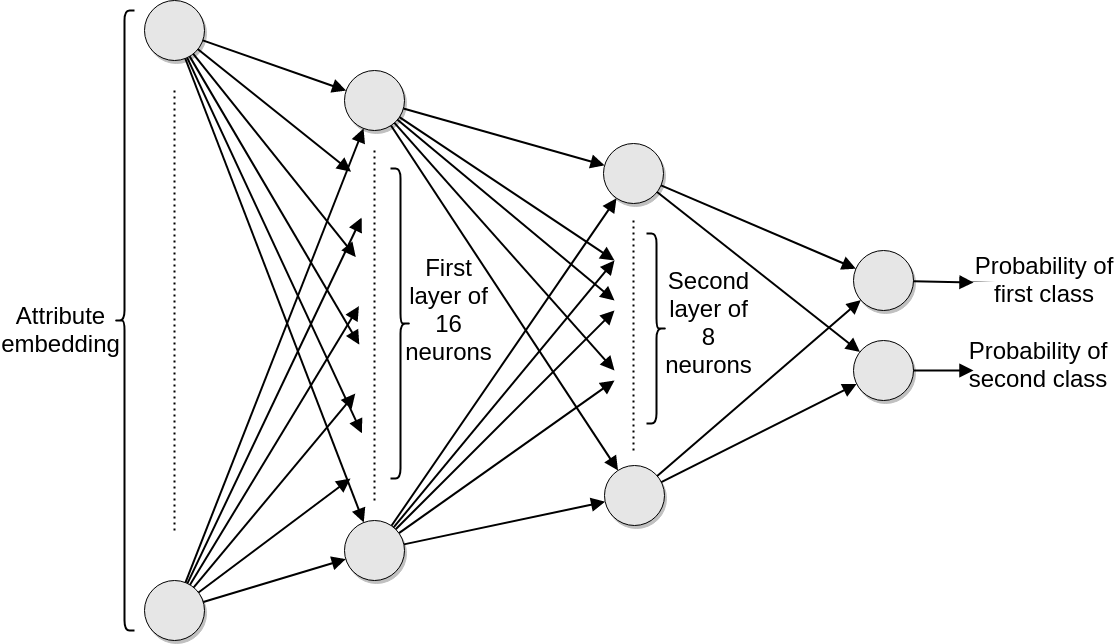
\includegraphics[width=\textwidth]{img/Bottom-level_NN}
\end{figure}

The \textit{sigmoid} activation function proved to be the most successful in all layers (\ref{eval:bottom-model-tuning}).
During the model training, an Adamax optimizer with learning rate of 0.02 was applied in 100 epochs and batch size of 10.
To prevent the overfitting, the model stopped learning in case of increasing loss on a validation set (10\% of training data).
The applied loss function is called the Cross Entropy (CE), which is defined as follows:
$$
H(P, Q) = -\EX_{x \sim P} \log{Q(x)} = -\sum_x P(x) \log{Q(x)}
$$
where $P$ is the true probability distribution and $Q$ is the predicted probability distribution over samples $x$ \cite{Goodfellow-et-al-2016}.
Note that the roles of true and predicted distributions are given, in contrast to the accuracy measure.

\section{Law-Case classifier}
\label{sec:law-case-classifier}
The goal of the Law-Case classifier is to assign a document to one of the classes: law-related or case-related.
As the Data Characteristics chapter (\ref{chp:data_characteristics}) defines the classes only loosely, the following paragraphs provide more specific and statistical definition.

Case-related documents contain at least one specific information about the subjects or acts related to the case. 
The authors of these documents are usually directly involved in the case or at least has come into contact with the subjects.
They are mostly confidential, such as emails, medical records, emergency call records, police records or testimonies.
Their main characteristic is an occurrence of a known entity, such as victim, defendant or location of an event that is part of the case.

Law-related documents do not contain any information specific to the case.
They usually state facts that help lawyers argue about the legal aspects of the case and find disagreement and evidence.
Examples of such documents are fragments of law code, description of similar cases from the past, policies of a company/school/office, news, books, or articles.
Their main characteristic is a specific vocabulary, usually including the legal terminology.

All 263 documents were labeled by one of the classes as part of the annotation process.
The case related group is in majority with 199 document versus 64 law-related documents (32\% of all).
This ratio implies that a model predicting all documents as case-relevant achieves accuracy of 0.68.
Further in the text, this simple model will be referred to as a baseline model.
Note that the evaluation metric inspected here is an accuracy score, in comparison with the relevance prediction where precision and recall are of interest.
The reason for that is the equal nature of the two classes -- one is not more important than the other.
To train the models, we had to establish a simplified assumption and mark all sentences with the same class as the document.
As a result, the models were trained on all 14,368 sentences.

The top-level model of Law-Case classifier is working with the following several sets of attributes.
The first set is extracted and used as an input for the bottom-level models: sentence meaning, keywords, relations and entities.
Their encoding is explained in the section \ref{sec:attributes}.
The second set contains the structural characteristics of the document as explained in the section \ref{sec:structural_characteristics}.
Next set of attributes is created by counting the entities that appear in the sentence.
The assumption is that the law-related documents do not contain as many entities as the case-related, since the explanation of laws uses neutral words, such as ``defendant'', ``subject'', ``suspect'', and similar.
Next two attributes are first and second level of categories.
The decision about including only first two levels was driven by the fact, that the third category was assigned to less than a half of the documents and the forth category to less than one tenth.
The last two attributes are derived from the concepts of documents.
First, the concepts are organized into two groups -- case concepts and law concepts -- such that the case concepts appear in some case-related document but not in any law-related and opposite is true for the law concepts.
Then, the attributes express the number of case and law concepts in the given document.

\begin{figure}[h]
\caption{Accuracies of bottom-layer models for prediction of case-related and law-related documents.}
\label{fig:Case-Law_accuracies}
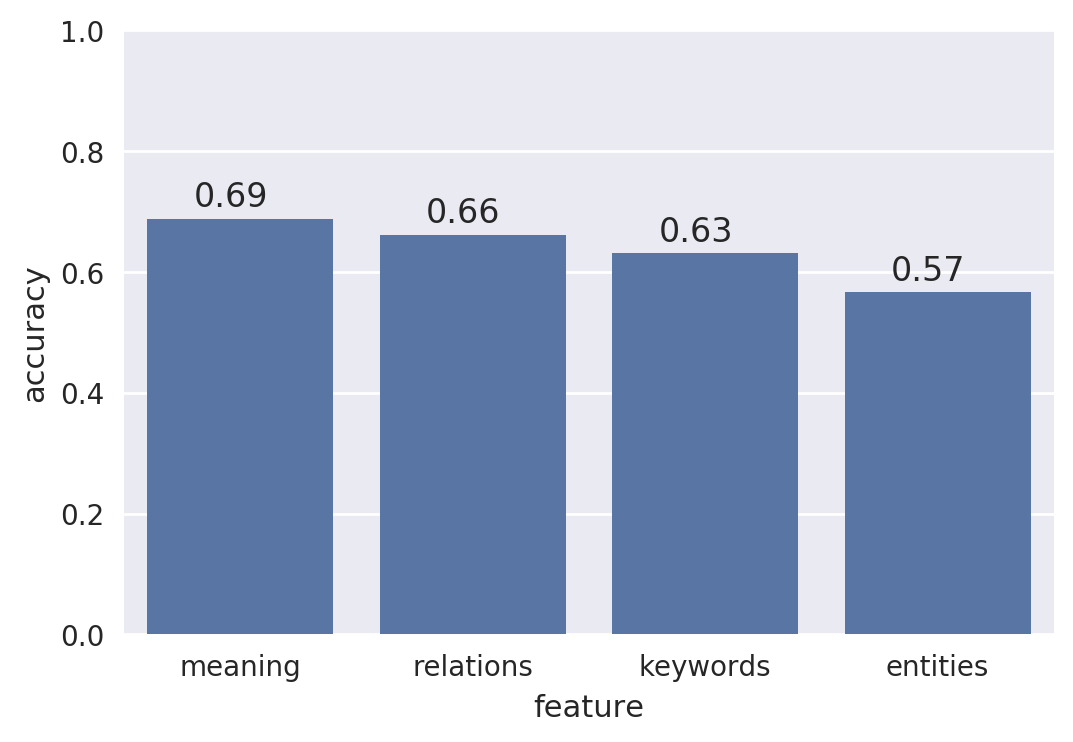
\includegraphics[width=0.9\textwidth]{img/Case-Law_accuracies}
\end{figure}

The figure \ref{fig:Case-Law_accuracies} reveals the accuracies of bottom-level classifiers in the task of predicting the class of documents.
The models were evaluated on each document after training on sentences of all other documents (Leave-One-Out method).
One can notice rather poor performance with \textit{meaning} the most discriminative attribute.
On the other hand, the \textit{entities} do not contribute very well to the predictions.
Even though the results suggest low performance of the top-level model too, the combination of bottom-level models turns up to be surprisingly powerful.

To determine which attributes are actually beneficial and which are irrelevant, one can plot the importances of individual features suggested by \textit{Random Forest} classifier.
The classifier computes \textit{gini index} \footnote{Measure of class impurity for determining the next feature to split on \\(\url{http://scikit-learn.org/stable/modules/tree.html\#tree}).} that not only drives the decision tree creation, but also signifies the feature importance.
The evaluation in the figure \ref{fig:case_law_feature_importance} takes advantage of this ability and displays the features sorted by its importance.

\begin{figure}[h]
\caption{Feature importance from Random tree decision classification of case-related and law-related}
\label{fig:case_law_feature_importance}
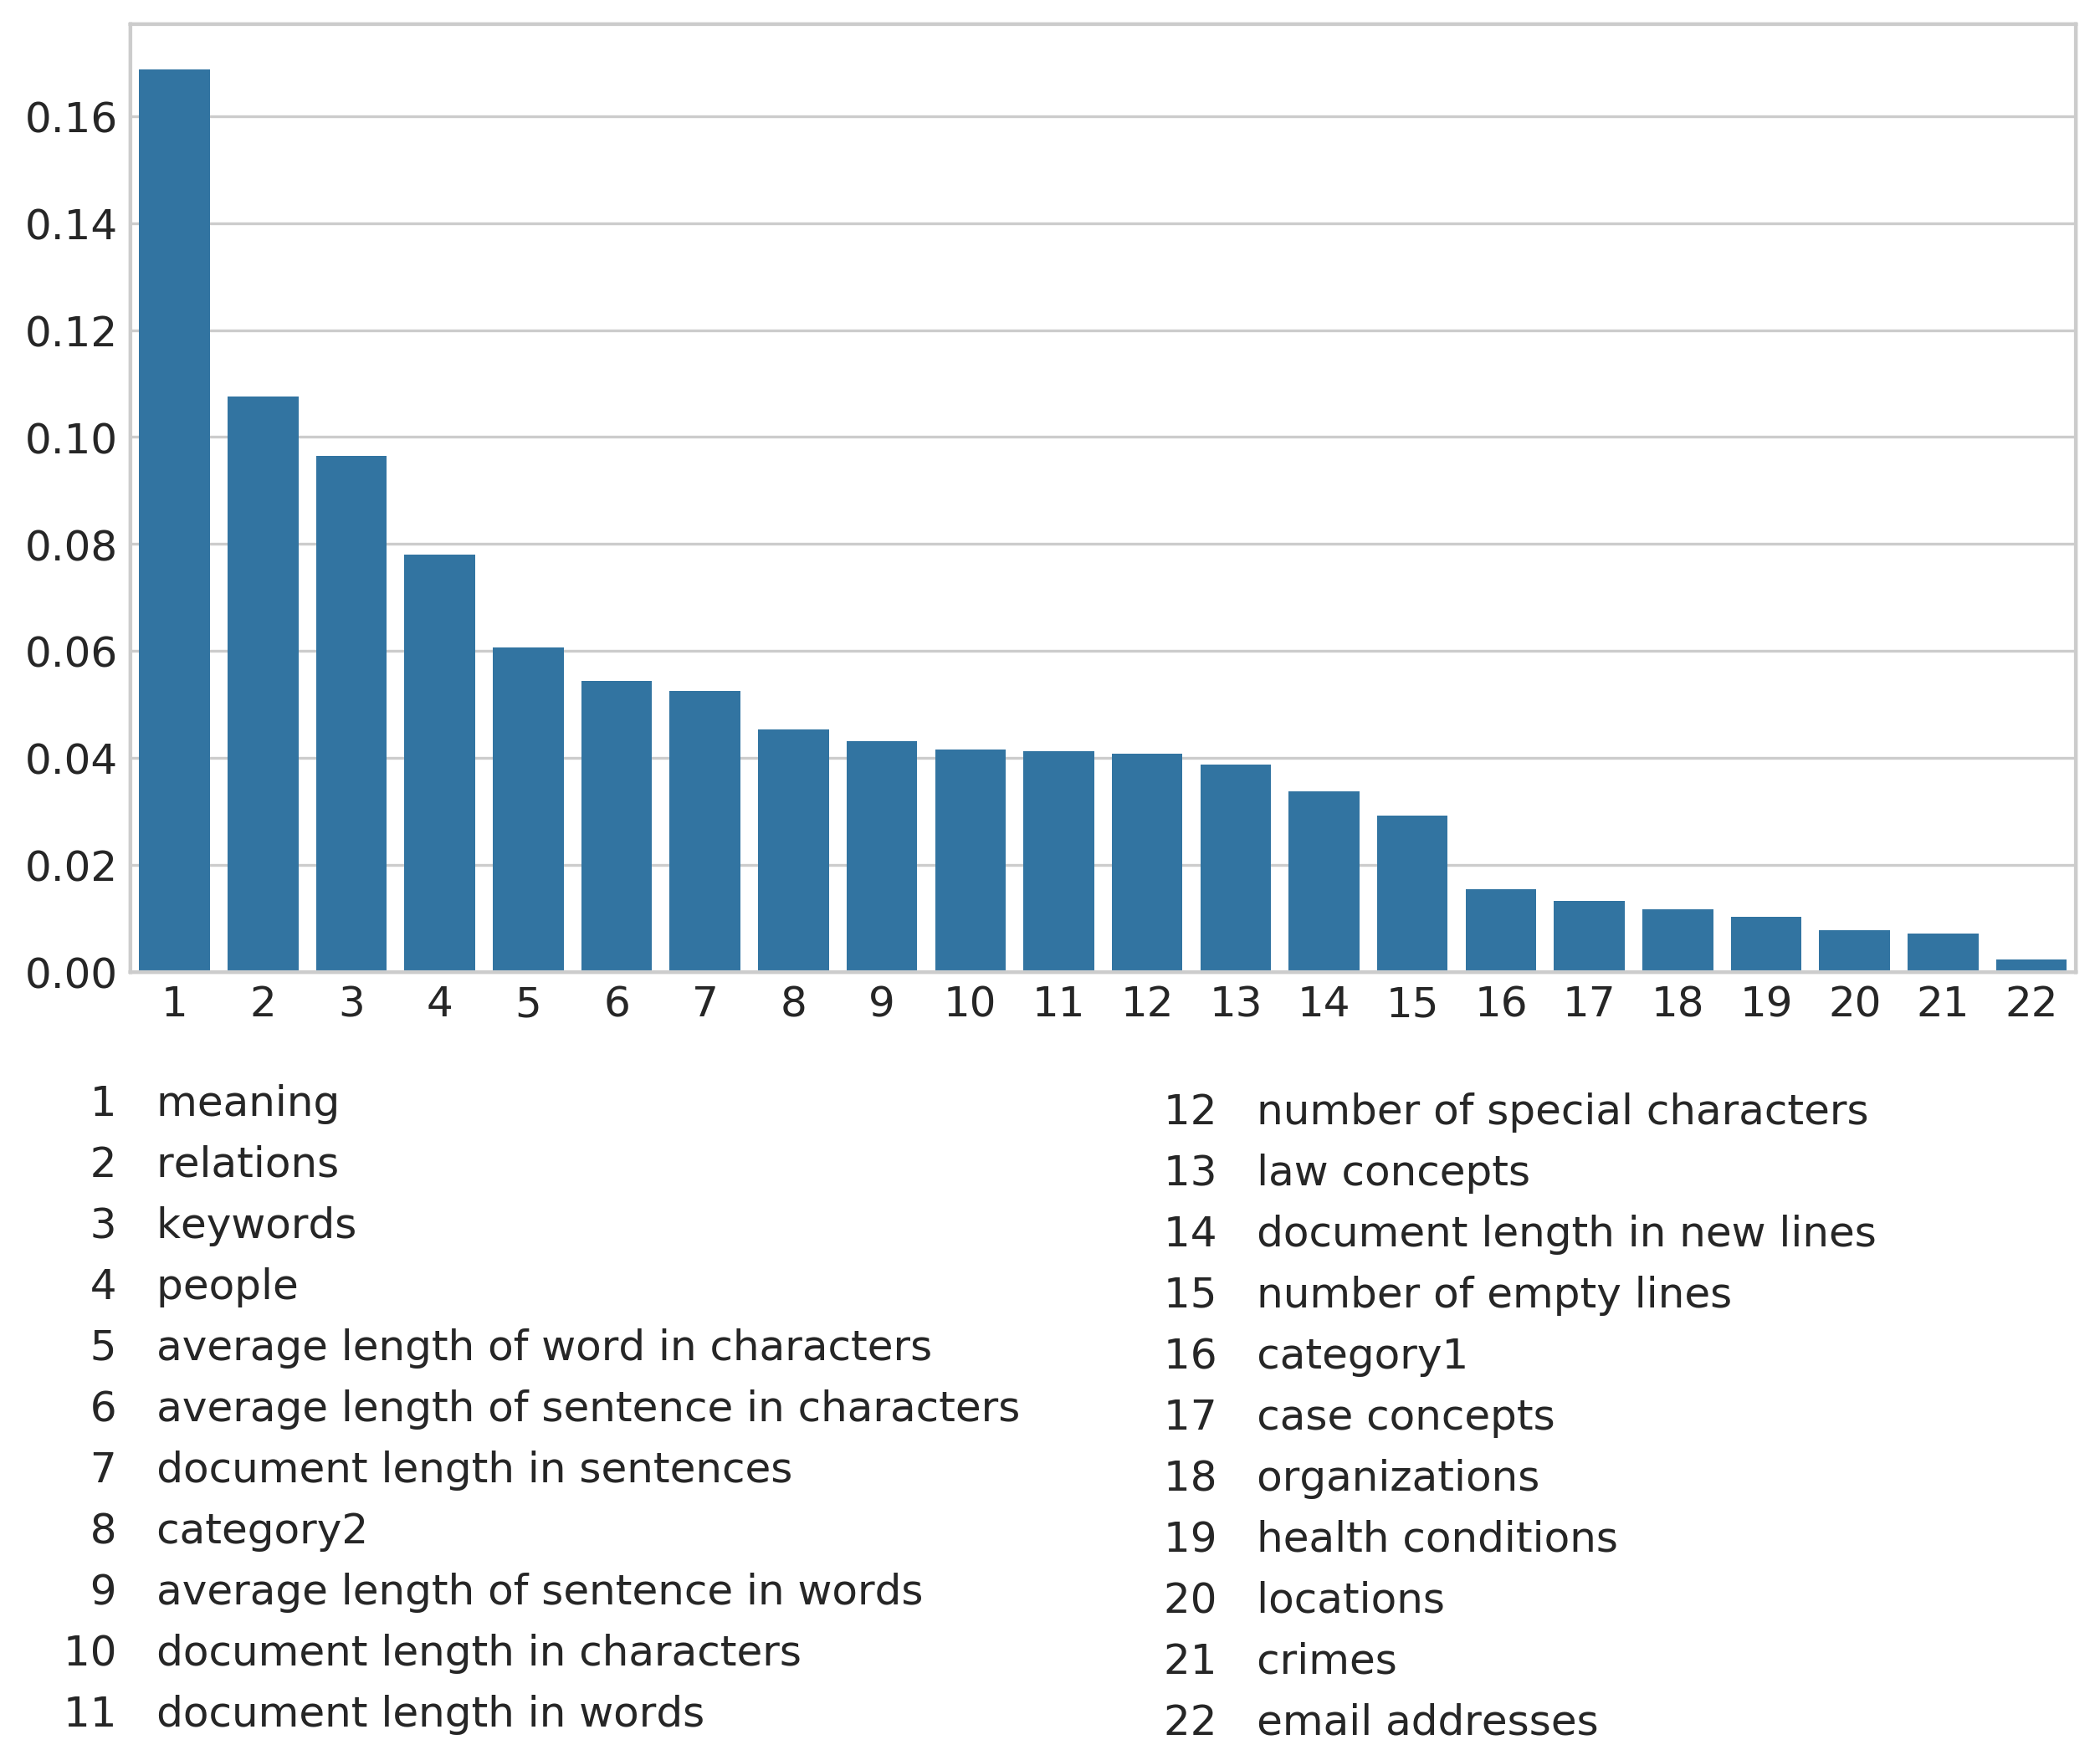
\includegraphics[width=\textwidth]{img/case_law_feature_importance}
\end{figure}

The first three most important features are occupied by the bottom-level models meaning, relations and keywords.
The entities model with its importance less than $0.03$ is useless in this settings and will not be considered in the final model.
Some of the structural characteristics are successful, such as average length of word of document length.
The significance of the word length might be caused by more detailed and professional terminology of law-related documents, which often includes longer words.
The document length feature might be influenced by the long case-related testimonies, which is a specific artifact of our data set.
Out of the entity counts, only the people were marked as important.
The others will not be considered in the final model.
Interestingly, the first level of category is not relevant as much as the second level.
This might be due to the general nature of the first level, which is probably sharing a single value for a large number of documents, and therefore, it looses the discriminative power.
The final model considers only the second level.
Regarding the concepts, they proved not to be very helpful in this classification task.

\begin{figure}[h]
\caption{Importance of dimensions in sentence meaning word2vec vectors}
\label{fig:vec_importance_caselaw}
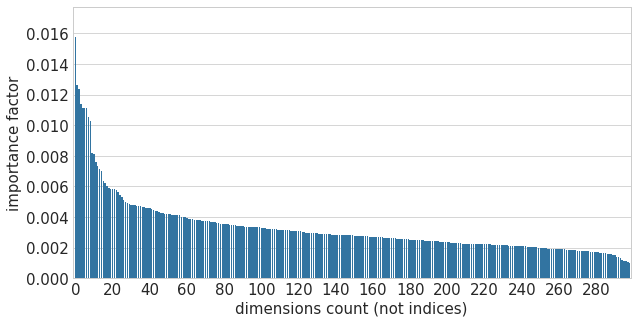
\includegraphics[width=\textwidth]{img/vec_importance_caselaw}
\end{figure}

As the most discriminative attribute is the meaning, the next two paragraphs describe the behavior of sample points (sentences) with respect to this attribute.
The figure \ref{fig:vec_importance_caselaw} shows the importance of each of the 300 dimensions of the vector.
The importance is following the Zipf's law, as the importance seems to be decreasing exponentially with the ordered dimensions.
Nevertheless, the dimensionality reduction did not help in the classification and the accuracy rather decreased.

\begin{figure}[h]
\caption{First 3 components of PCA analysis plotted with labels according to the case and law related sentences}
\label{fig:PCA_caselaw}
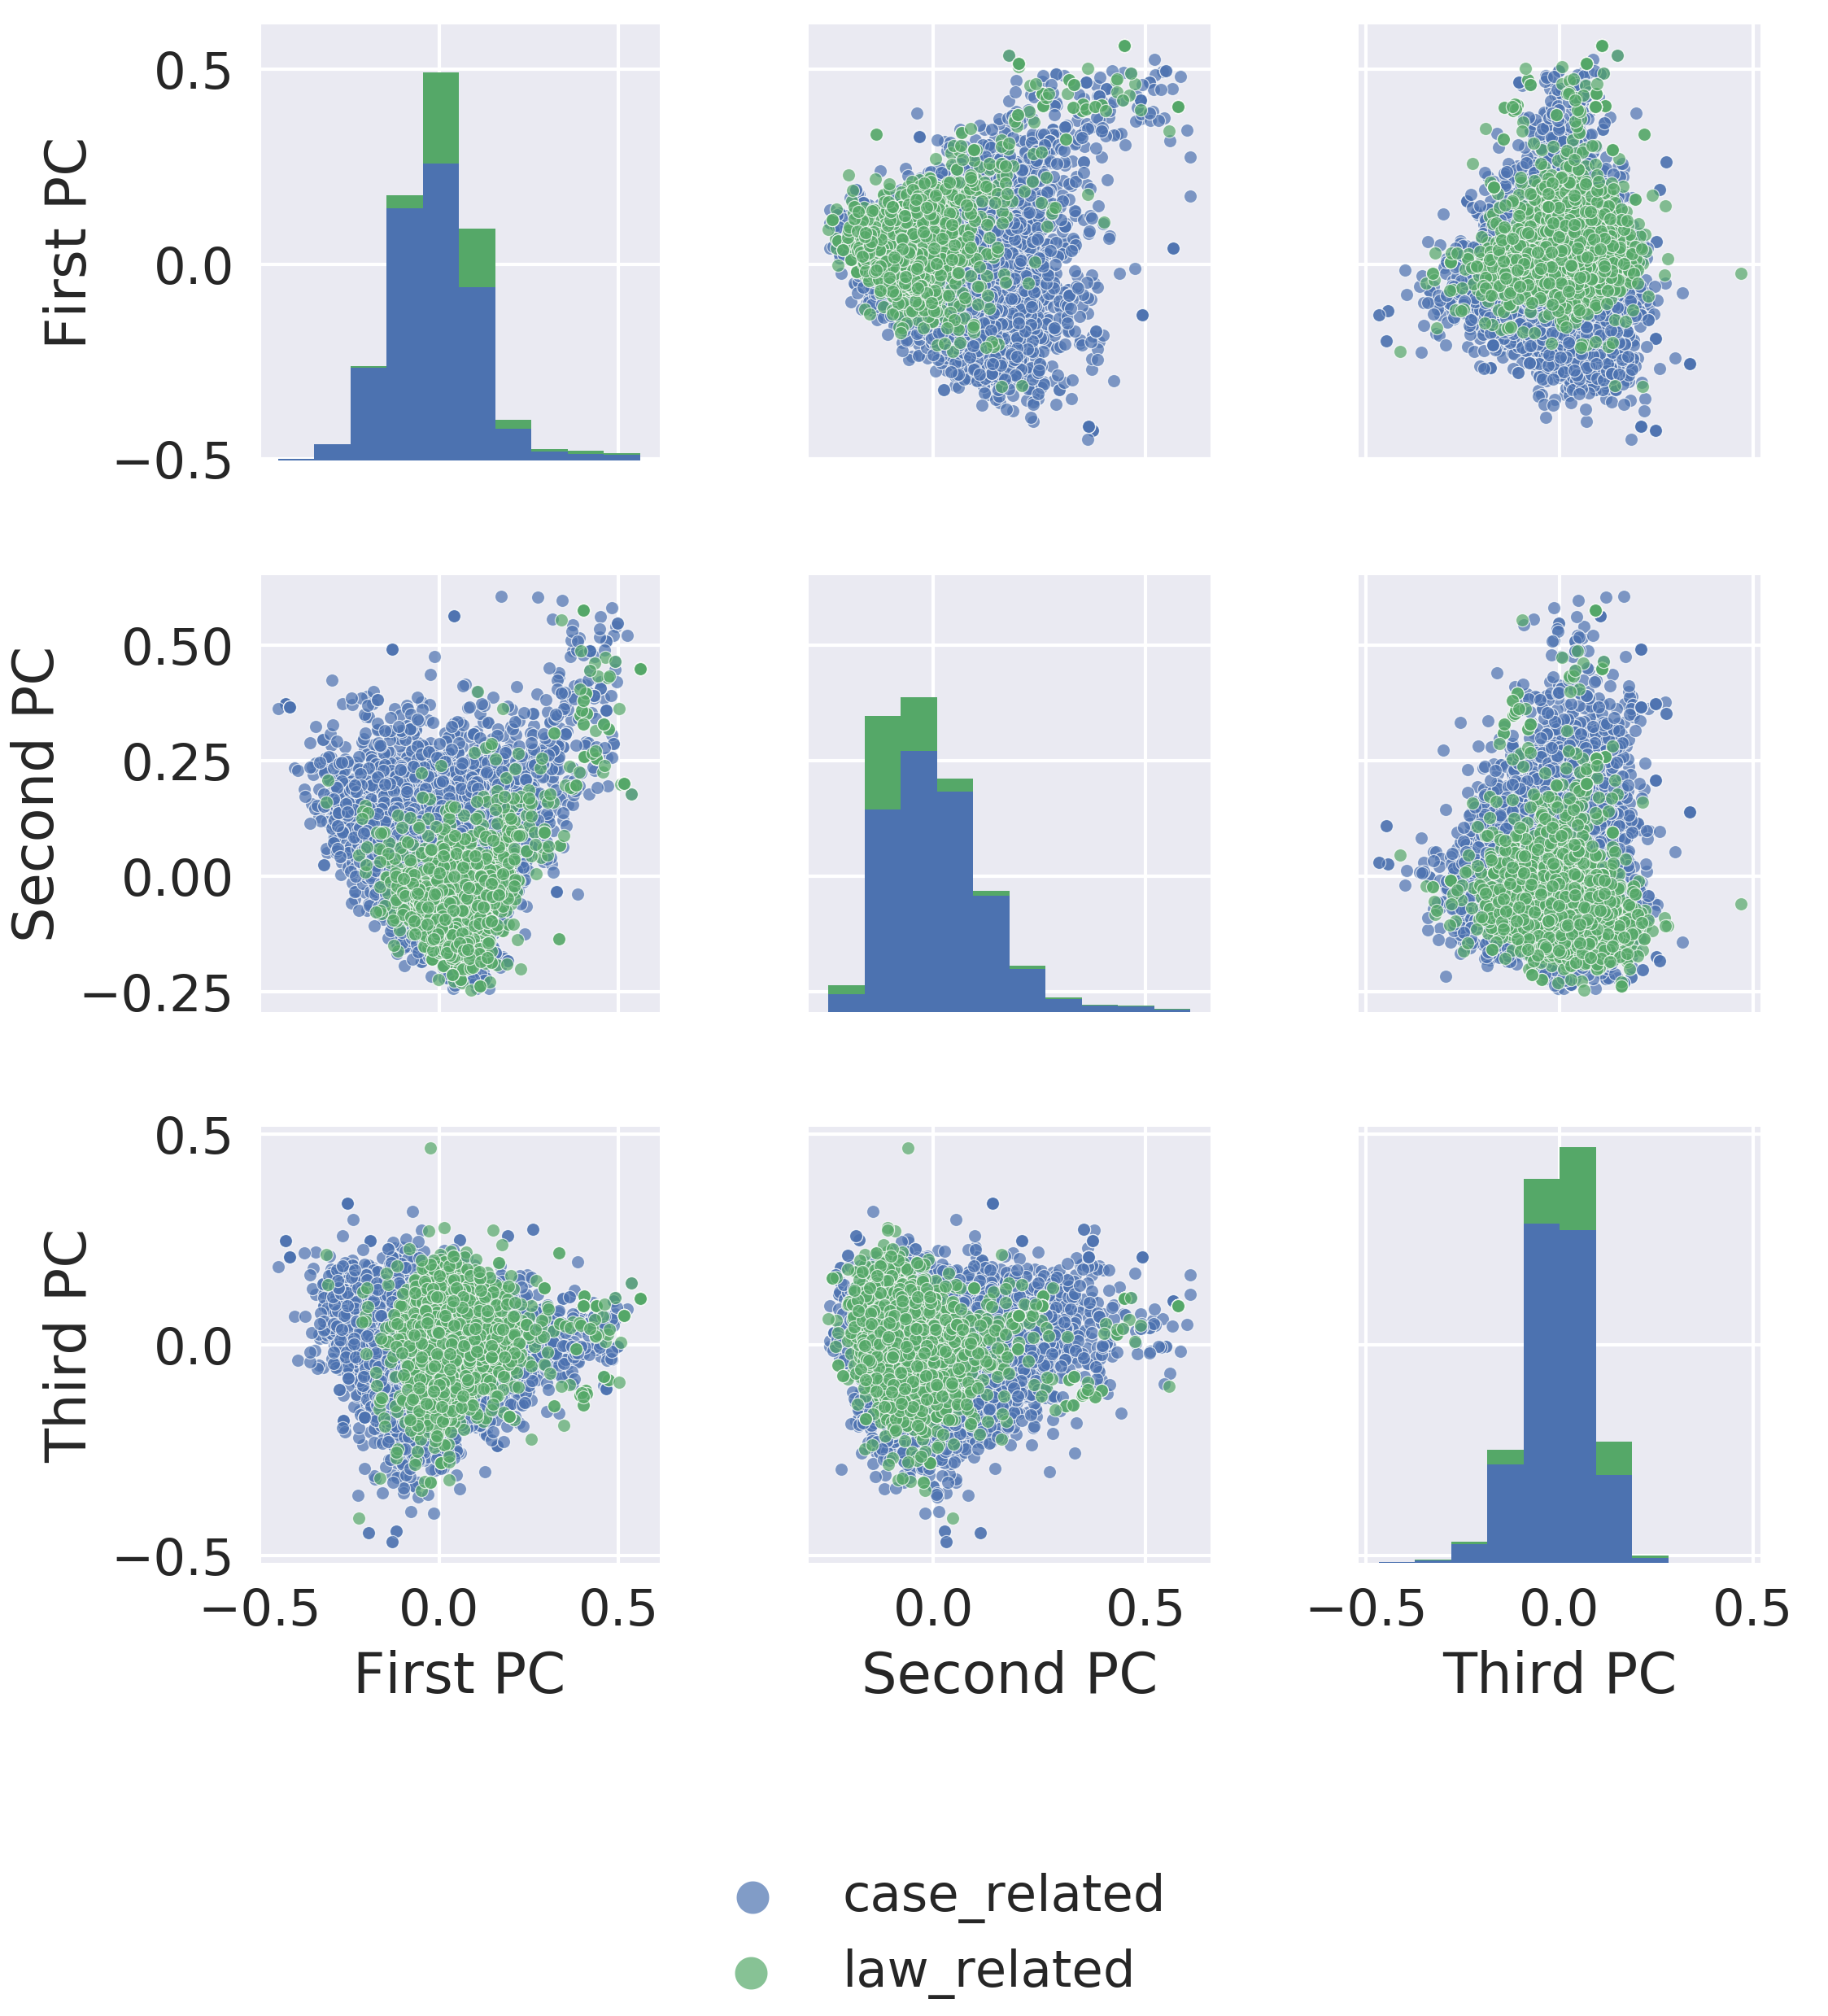
\includegraphics[width=\textwidth]{img/PCA_caselaw}
\end{figure}

Next plot (\ref{fig:PCA_caselaw}) shows sentences plotted pairwise according to the first three principal components of the meaning attribute.
It might seem that the law-related documents are located at the center and the case-related documents are more spread.
However, this impression might be influenced by the fact, that there is three times fewer law-related documents.
In any case, the data keep triangular shape with one corner more populated by case-related documents, which might be the reason for the success of the meaning attribute.


The top-level model is based on the first 12 features in the figure \ref{fig:case_law_feature_importance}.
In this case, the model is trained on the set of documents, which has only 263 instances, hence the neural networks are not applicable.
As the best classifier showed to be the \textit{Random Forest} (\ref{eval:law-case-model-selection}) with 20 base estimators and maximum tree depth of 7 (\ref{eval:law-case-model-tuning}). The final model achieved performance of $0.89$ on the set of all documents with Leave-One-Out method. Now, when the division to the two diverse types of documents is in place, the labeled documents can proceed to the relevance prediction.
Note that we will train the following classifiers separately according to the true case-related and law-related labels.

\section{Sentence relevance classifier}
\label{sec:sentence-classifier}
The sentence relevance prediction is relatively harder task than the previous classification.
Humans consider sentences relevant based on different factors.
For the sake of simplicity, the system assumes the relevance depends on the words that appear in the sentence, especially keywords.
In reality, the context of the document, case, and other external knowledge plays a significant role, which is ignored here.
Another factor that makes the prediction difficult relates to the process of human annotation: in case there are multiple sentences with relevant information, a lawyer would highlight only one of them as important.
As a result, the model trains on a dataset, where similar sentence appears as relevant and irrelevant at the same time.


Instead of the accuracy, the observed evaluation score is now precision and recall.
The precision expresses a percentage of correctly classified sentences out of all sentences that was classified as relevant.
The recall expresses a percentage of correctly classified sentences out of all relevant sentences.
As mentioned in the section \ref{sec:related_relevance}, the recall is usually more valued in the E-discovery, since the extra time of the lawyer spent on an irrelevant piece of information outbalance the situation, in which the lawyer is not notified about some relevant information.
The section mentions the human performance in evaluating the relevance: precision ca 20\% and recall ca 50\%.
These values set a baseline in the following experiments.

Two groups of attributes are applied in the sentence predictions: general and case-specific. 
The general attributes are trained on full set of documents and there is only one model for every case.
Its purpose is to explain the general trends of the relevance.
On the other hand, the case-specific attributes are trained on documents of only the same case and they are expressing the case-specific relevance.

\subsection{General attributes}
The general attributes include the \textit{word2vec} vectors: meaning, keywords and relations.
The entities vector proved to be inefficient in the Law-Case model, therefore, it is not considered here.
The bottom-level models (\ref{sec:bottom-level-models}) are applied to train the sentence relevance.
For each document, the models were trained on all other documents and the sentences were assigned a probability, that it is relevant.
This setting expects, that in the time of prediction, all other documents of the case are already uploaded.

Thanks to the predicted probability, there is a straightforward tool to trade between the precision and recall.
Let us define a parameter $p$ as the minimum probability for a sentence to be considered as relevant.
With increasing $p$, the recall increases and precision decreases.

The figure \ref{fig:sent_PandR} shows the precisions and recalls for all three general attributes with respect to the parameter $p$.
Obviously, the keywords and relations failed to learn the features well, because the precision never increases with higher $p$.
In contrast, the figure \ref{fig:sent_meaningP} indicates a more promising situation.
For $p=0.5$, the model achieved more than 20\% of precision and crossed the 50\% of recall, which is the aforementioned human performance.

\begin{figure}[h]
\begin{subfigure}{.5\textwidth}
  \centering
  \caption{Meaning attribute}
  \label{fig:sent_meaningP}
  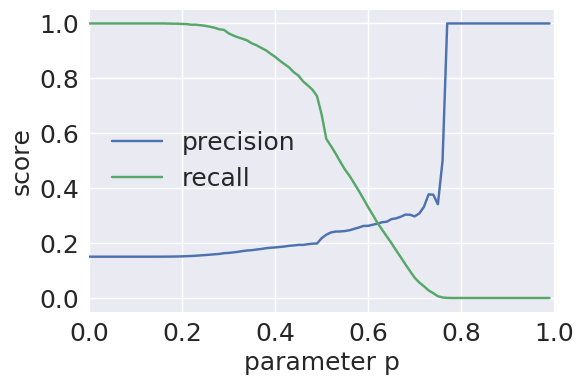
\includegraphics[width=\textwidth]{img/sent_meaningP}
\end{subfigure}%
\begin{subfigure}{.5\textwidth}
  \centering
  \caption{Keywords attribute}
  \label{fig:sent_keywordsP}
  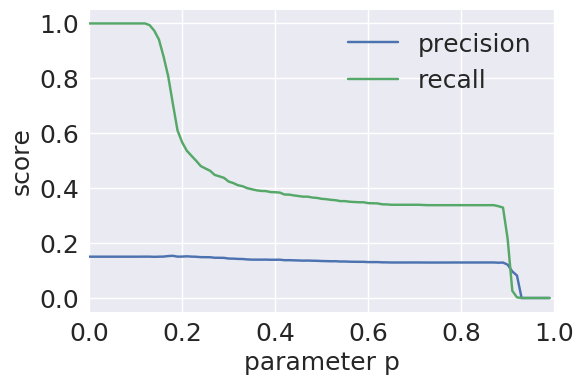
\includegraphics[width=\textwidth]{img/sent_keywordsP}
\end{subfigure}%
\\
\begin{subfigure}{.5\textwidth}
  \centering
  \caption{Relations attribute}
  \label{fig:sent_relationsP}
  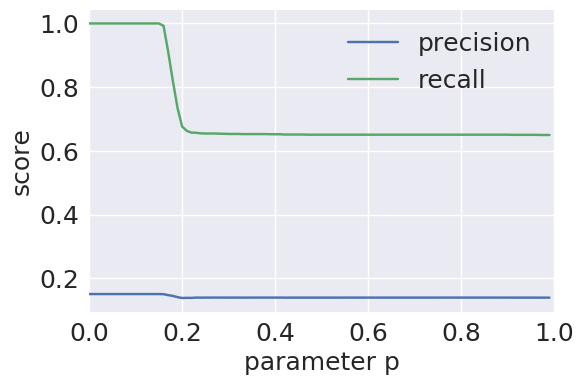
\includegraphics[width=\textwidth]{img/sent_relationsP}
\end{subfigure}
\caption{Precision and recall of the general attributes}
\label{fig:sent_PandR}
\end{figure}

Surprisingly, the meaning is again the superior attribute (similarly as in the Law-case classifier).
It seems that the neural network does not really need to pick keywords or any other subattributes in the text, as it is able to extract them itself.
This fact 
\begin{figure}[H]
\caption{First 3 components of PCA analysis plotted with labels according to the sentence relevance}
\label{fig:PCA_sent_relevance}
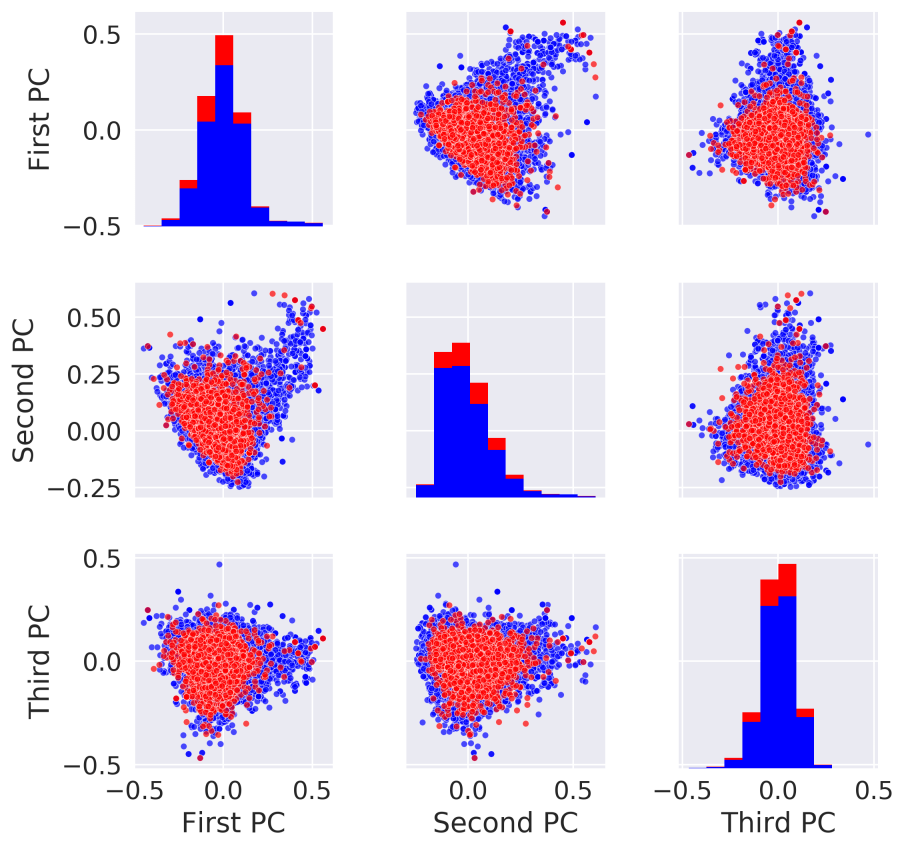
\includegraphics[width=\textwidth]{img/PCA_sent_relevance}
\end{figure}

\subsection{Case-specific attributes}
% describe how they are created in case-preprocessor, vectors in sentences




\section{Document relevance classifier}
\label{sec:document-classifier}
[Law-Document and Case-Document classifier]

\begin{figure}[H]
\caption{First 3 components of PCA analysis applied on sentence meanings with labels according to the document relevance}
\label{fig:PCA_sent_relevance}
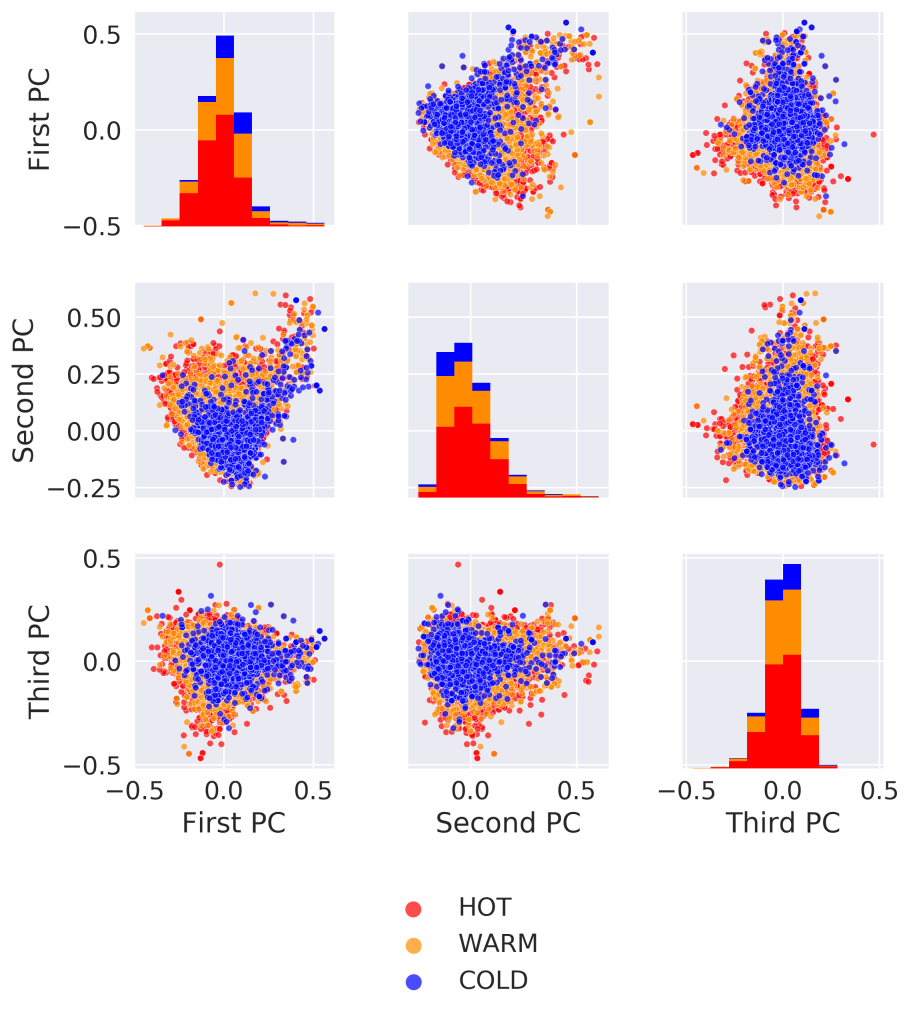
\includegraphics[width=\textwidth]{img/PCA_doc_relevance}
\end{figure}

\chapter{Implementation}
Based on the research introduced in the previous chapters, a system for Classification of LAW Documents (Clawd) was designed and developed.
Its purpose is to process textual information about legal cases, documents, and other user's inputs, pass the raw data to NLP services to extract features and evaluate relevance of the documents and its individual sentences.
Clawd is a stand-alone web application independent of Legato, though Legato is the only system communicating with Clawd so far.
The first section introduces the development tools, second explains the design and the last describes how Legato and Clawd are integrated.

\section{Frameworks and libraries}
The application is written completely in Python 3.4 following the PEP 8 style guide\footnote{Python coding conventions (\url{https://www.python.org/dev/peps/pep-0008/})}.
As a web application framework, \textit{Django}\footnote{Python web framework (\url{https://www.djangoproject.com/})} has been applied.
Besides the web interface, \textit{Django} provides many other features that ease the development and keep the architecture clear.
For example, it manages database, logging, tests, security, caching, etc.

% MongoDB
The main decision about the database was between the relational and NoSQL database.
Generally, the NoSQL databases are beneficial when either the database needs to be heavily distributed or the data are expected to be loosely defined without strict internal structure.
The former is not this case but the latter applies.
As the output of the NLP services is formated to a complex JSON, especially the entity relations, the structure of data is highly variable.
Apart from that, the Clawd is indulgent in the choice of NLP services, which means there might be other data structures added in the future.
To ensure the structure flexibility, Clawd stores the data in a NoSQL database specifically, \textit{MongoDB}.

% NLP tools
The following tools have been applied to process the text:
\textit{NLTK}\footnote{Natural Language Toolkit for Python \url{http://www.nltk.org/}} library helps to split the text into sentences, remove stopwords and compute the TF-IDF score, 
\textit{Gensim}\footnote{Topic modeling library \url{https://radimrehurek.com/gensim/}} provided a fast data structure for Word2vec vectors retrieval, \textit{datefinder}\footnote{Library for date extraction \url{http://datefinder.readthedocs.io/en/latest/}}
helps extract dates from text and, finally,
Watson Developer Cloud\footnote{Watson Services API \url{https://pypi.org/project/watson-developer-cloud/}}, which provided communication with \textit{Watson NLU} service to extract the most important features.
The scientific computations and machine learning modeling is handled by \textit{Numpy}\footnote{Package for scientific computing \url{http://www.numpy.org/}}, which provides fast scientific computing,
\textit{Pandas}\footnote{Python data analysis library \url{https://pandas.pydata.org/}}, which helps with exploratory data analysis,
\textit{Scikit-learn}\footnote{Machine learning library \url{http://scikit-learn.org}}, which offers machine learning models and tools for their evaluation and
\textit{Keras}\footnote{Neural network library \url{https://keras.io}} library, that enables high-level design of neural networks in Python.

% celery, apache
The application often needs to trigger time demanding tasks (neural networks learning, network communication, and text processing), despite the fact that the communication with Legato takes place in the meantime and all responses from Clawd must be immediate.
For this reason, the tasks need to be organized in asynchronous queues, which is handled by the \textit{Celery} framework\footnote{Distributed task queue \url{http://www.celeryproject.org/}}.

The web application is deployed on a \textit{Debian} server\footnote{Linux operating system \url{https://www.debian.org/}} inside the \textit{Apache} web container\footnote{HTTP server for modern operating systems \url{https://httpd.apache.org/}}.
All communication with NLP services and Legato takes place in JSON format through HTTP protocol.

\section{Design and implementation}
Clawd is designed in three layers, as shown in the figure \ref{fig:Design}: the view layer (API), service layer and asynchronous task queue \textit{Celery}.
Legato requests are served by the API, which passes the data to the service layer.
If there are any time-demanding tasks, the service layer passes data to \textit{Celery} to be processed asynchronously.
Quick tasks are computed by the service layer immediately and the answer is passed back to the API to return the response.

\begin{figure}[h]
\caption{Design of the Clawd system}
\label{fig:Design}
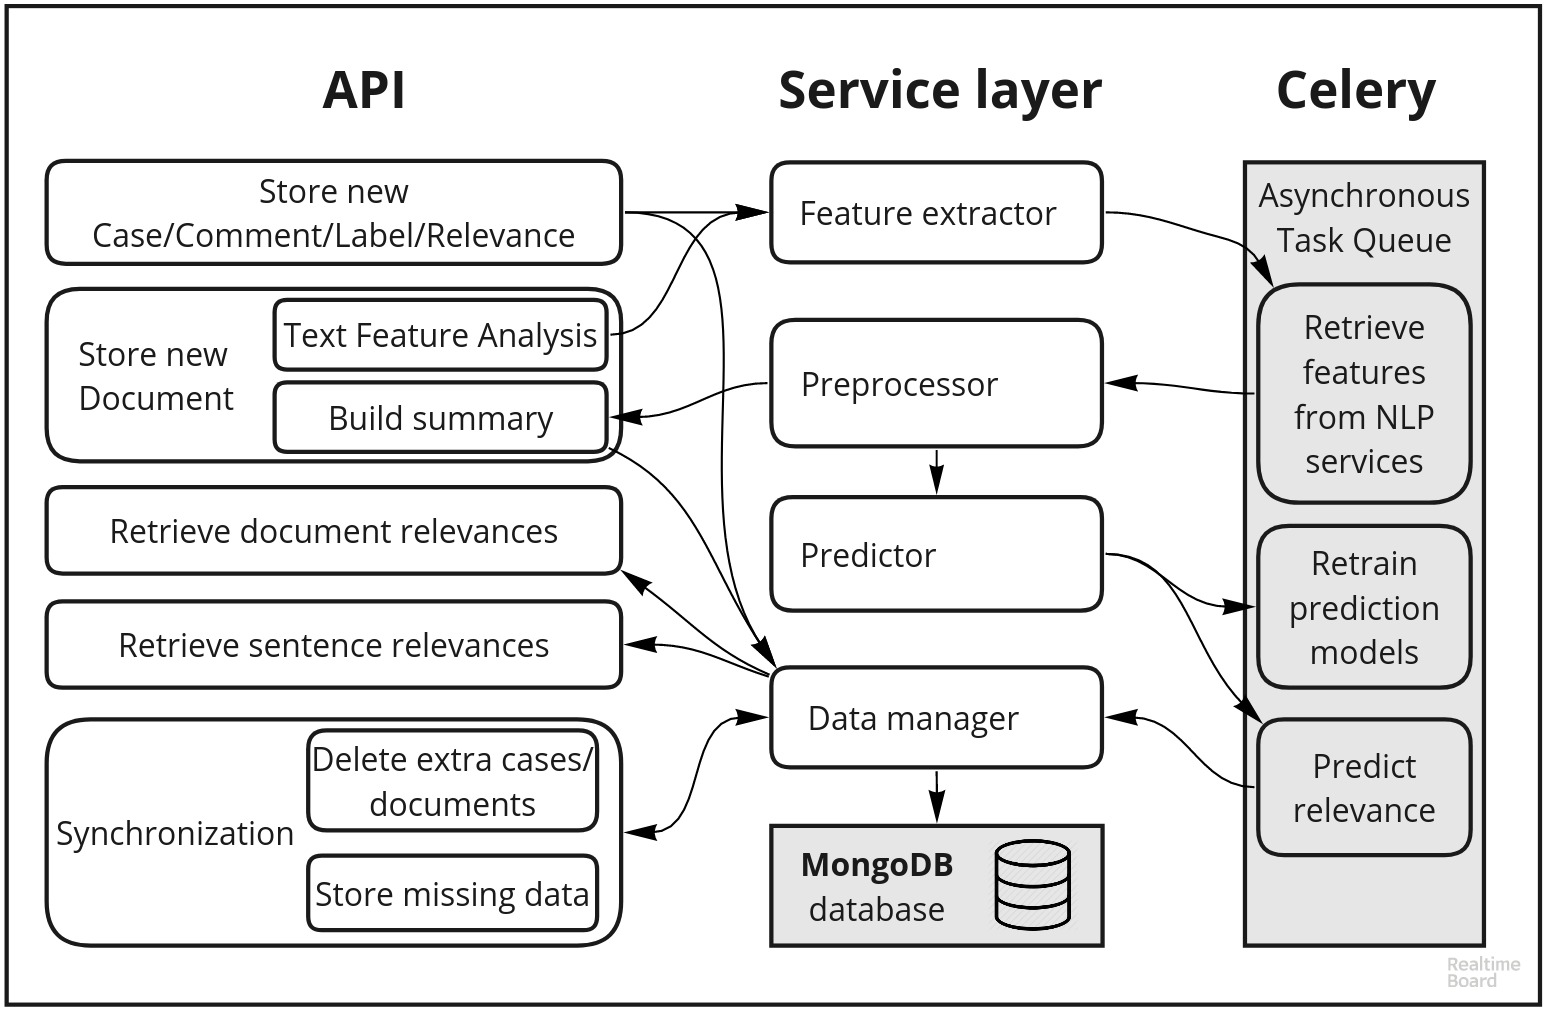
\includegraphics[width=\textwidth]{img/Design}
\end{figure}

\subsection{Application Programming Interface}
\label{sec:api}
The three main use cases of Clawd are 1) Storing a new case, comment, label or relevance -- in all these scenarios, the information is stored and models updated to yield new relevances, 2) Storing a new document -- here, the text is sent to the NLP services, text is preprocessed, models updated and summary is built and returned to Legato, and finally 3) Relevance retrieval -- in this case, no computations take place and the relevances stored in Clawd are returned.
One extra use case, which is not initiated by user, is the synchronization step, that ensures the data in Clawd are consistent with data in Legato.

The documentation of Clawd's API is described in the table \ref{fig:api}.
The interface is following the REST API guidelines.

\begin{figure}[h]
\centering
\caption{Application programming interface of Clawd}
\label{fig:api}
\begin{tabular}{|m{2cm}|m{5.5cm}|m{5cm}|}
\hline
\rowcolor{gray!30}
\textbf{Method} &  \textbf{Endpoint}   &  \vspace{0.2cm} \textbf{Description}   \\[10pt] \hline
GET  &  /case/\{\textit{caseId}\} & Retrieve information about the case. \\ \hline
POST  & /case/\{\textit{caseId}\} & Creates a new case or updates existing. \\ \hline
DELETE  & /case/\{\textit{caseId}\} & Deletes a case.  \\[6pt] \hline
GET  & /case/\{\textit{caseId}\}/doc/\{\textit{docId}\} & Retrieve information about document. \\ \hline
POST  & /case/\{\textit{caseId}\}/doc/\{\textit{docId}\} & Creates new document or updates existing. \\ \hline
DELETE  & /case/\{\textit{caseId}\}/doc/\{\textit{docId}\} & Deletes a document. \\[6pt] \hline
GET  & /case/\{\textit{caseId}\}/doc/\{\textit{docId}\}/\par relevance & Retrieve relevance of the document. \\ \hline
POST  & /case/\{\textit{caseId}\}/doc/\{\textit{docId}\}/\par relevance & Stores user relevance of the document.\\ \hline
GET  & /case/\{\textit{caseId}\}/doc/\{\textit{docId}\}/\par sent\_relevance & Get relevances of document's sentences.\\ \hline
GET  & /case/\{\textit{caseId}\}/doc/\{\textit{docId}\}/\par label & Retrieve label of the specified document. \\ \hline
POST  & /case/\{\textit{caseId}\}/doc/\{\textit{docId}\}/\par label & Stores label of the specified document. \\ \hline
GET  & /case/\{\textit{caseId}\}/doc/\{\textit{docId}\}/\par comment/\{\textit{commentId}\} & Retrieve comment of the document. \\ \hline
POST  & /case/\{\textit{caseId}\}/doc/\{\textit{docId}\}/\par comment/\{\textit{commentId}\} & Stores comment on the document. \\ \hline
GET  & /case/\{\textit{caseId}\}/relevances & Retrieve relevances for all documents of the case. \\ \hline
GET  & /sync\_proposal & Returns true if the synchronization is required. \\ \hline
GET  & /sync & Synchronization of the database with Legato. \\ \hline
\end{tabular}
\end{figure}

\subsection{Service layer}
The Django applications are a natural way to achieve modularization of an application in Python.
The service layer takes advantage of this feature and splits its functionality into four modules.

The \textit{Feature extractor} module abstracts the rest of the application from the specific NLP services and implements their individual API's.
It also computes other features that does not need to be extracted by remote service, but rather processed by a local library -- this is a case of date extraction.
All features are stored in the database to be further processed by other modules.

The \textit{Preprocessor} module applies the text preprocessing and attribute extraction as explained in the section \ref{sec:attributes}.
The module also includes several dictionaries, such as \textit{Word2vec} or list of \textit{Watson} types of relations or entities, which are required to compute the attributes.

The \textit{Predictor} module keeps track of all the models needed for prediction.
For each case, it tracks bottom-level models for each attribute and two top-level models: for sentence and case classification.
All tasks of \textit{Predictor} are time-demanding, therefore, they are all passed to the \textit{Celery}.

The \textit{Data manager} keeps track of all data models in Clawd.
Thanks to the ORM\footnote{Object-Relational Mapping -- automatic mapping of application objects to database entities} provided by Django, the module is able to abstract from the underlying database and define data models in a natural Python way of defining classes.
The data models include Case, Doc, Sentence, Feature, Entity, Keyword, and Classifier.
All classifiers must be stored in a binary form.

\subsection{Celery}
The Celery handles a task management, but the execution itself runs on an implementation of so-called \textit{message broker}\footnote{\url{http://docs.celeryproject.org/en/latest/getting-started/brokers/}}.
Even though the most common message brokers are \textit{RabbitMQ}\footnote{\url{https://www.rabbitmq.com/}}, \textit{Redis}, or \textit{Amazon SQS}\footnote{\url{https://aws.amazon.com/sqs/}}, Clawd uses \textit{MongoDB} instead.
The reason is that the \textit{MongoDB} is already applied as the main data storage, and therefore, a new framework was considered unnecessary.

\textit{Celery} manages tasks with network communication, training of the models and evaluating relevance on models.
The tasks are being executed in multiple workers, which significantly increases the system's responsiveness.
The efficiency is especially noticeable in case of an initial synchronization, when all data are passed from Legato to an empty Clawd.


\section{Integration into Legato}
As mentioned earlier, Clawd is a stand-alone application that is integrated with Legato through the exposed REST API.
The communication was designed to be one-way only, hence all actions are initiated by Legato.
The only results from Clawd visible by a user are the suggested relevances and the document's summary.
Unfortunately, the Legato is not able to process and show sentence relevances so far, though Clawd provides the data.

The section \ref{sec:api} describes three use cases of Clawd, plus synchronization.
The first use cases (creation of a new case, comment, label, or relevance, and the relevance retrieval) is straight-forward, because the communication is simple storing of data in Clawd.
When Legato stores some of the aforementioned objects, it simultaneously sends them to Clawd.

The second use case (new document) is more sophisticated.
The figure \ref{fig:integration_new_file} shows a sequence diagram of the communication among not only Legato and Clawd, but also the user, Watson NLU service and Celery.
When a new document\footnote{The same data object is called \textit{File} in Legato and \textit{Document} in Clawd} is uploaded into Legato, a pipeline of preprocessing steps (explained in section \ref{sec:legato_usecase}) is applied.
One of the steps is also a summary extraction by Clawd.
When Clawd receives the document, it passes the data to Watson NLU service to extract features and stores the data from response.
Next, Clawd builds the document summary from the features and answers to Legato, which is now able to include the summary into document's view.
In the meantime, Clawd triggers follow-up tasks, which are processed by Clawd and include training of models and updating relevance.
Note that in this case, the request to Watson was not handled by Celery, as the Legato waits for the response and so, the communication must be synchronous (Celery handles only asynchronous tasks).

\begin{figure}[h]
\caption{Integration with Legato -- New File sequence diagram}
\label{fig:integration_new_file}
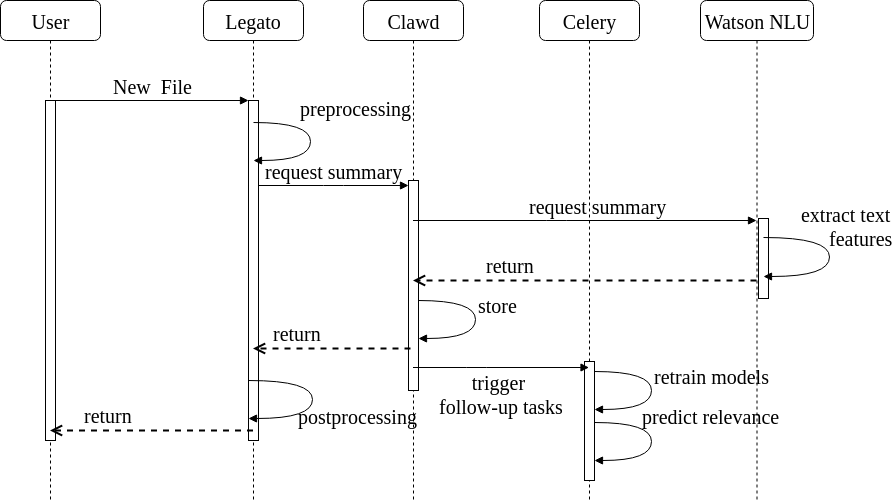
\includegraphics[width=\textwidth]{img/integration_new_file}
\end{figure}

The third use case is a request for computed relevances.
The main case dashboard in Legato contains a button for automatic relevance evaluation.
If a user chooses to click on it, the relevances are requested from Clawd, processed by Legato, and shown on the document's view page, as can be seen in the figure \ref{fig:integration_documentsview}.
User's own choices of relevances are shown in the left column and the predicted relevances are in the right column to enable comparison.

\begin{figure}[h]
\caption{Integration with Legato -- Document's view of real and suggested relevances}
\label{fig:integration_documentsview}
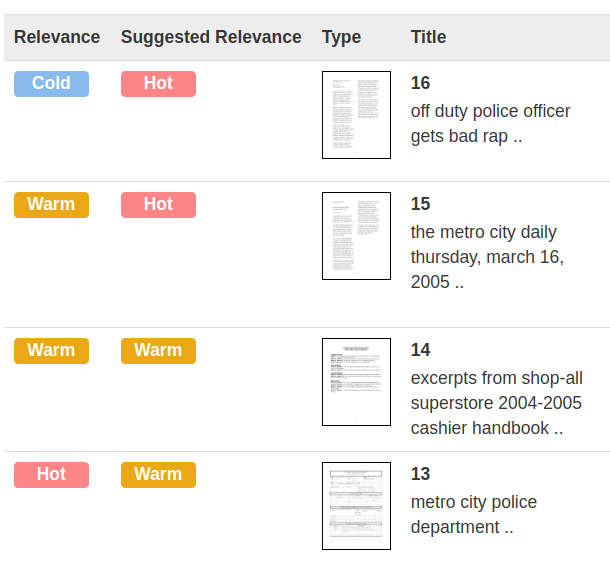
\includegraphics[width=0.8\textwidth]{img/integration_documentsview}
\end{figure}

The synchronization is an additional use case, which is, however, not triggered by a user.
Legato checks with Clawd after some period of time (usually one day), if the data are complete and up to date.
The process is initiated by Legato, which sends a list of identifications of all cases and documents.
Clawd deletes the extra objects not present in the list and answers with list of missing objects' identifications.
The last step is a transfer of all missing data from Legato to Clawd.

The working instance of Legato that is integrated with Clawd is accessible for public on 
\begin{quote}
\begin{tabular}{|>{\centering\arraybackslash} m{10cm}|}
\hline
\vspace{2mm}
\url{https://ai.demo.legato.sde.cz}
\vspace{2mm}
\hrulefill
\end{tabular}
\end{quote}
with login \textit{clawd@gmail.com} and password \textit{clawd}.
Users are free to create new cases and upload their own documents to evaluate the relevance.



\chapter{Evaluation}
\label{chp:evaluation}

\section{Decision point evaluation}

\subsection{Topology system of models}
% popsat ze jsem zkusil pouzit features primo z celeho dokumentu, ale uspesnost byla nizsi nez pri pouziti vet a pak dokument

\subsection{Bottom-level model selection}
\label{eval:bottom-model-selection}
% Law-Case classification based on Sentence Meaning
% ...Neural Networks        0.860
% ...SVM C=1.0              0.754
% ...RF n_est=500 depth=20  0.845

\subsection{Law-Case estimator selection}
\label{eval:law-case-model-selection}
After all values of attributes from bottom-level models were pre-computed, the next step was to pick the best top-level estimator.
The setting is the following:
\begin{enumerate}
\item low number of samples
\item low number of features
\item binary class
\item quantitative and ordinal features
\end{enumerate}
This combination of features suggests that decision trees or their ensembles could be the best suited.
Neural networks need more samples and SVM works best with a large number of features.
The figure \ref{fig:eval_law-case-model-selection} shows the comparison.

\begin{figure}[h]
\caption{Estimator selection for case-related or law-related classification}
\label{fig:eval_law-case-model-selection}
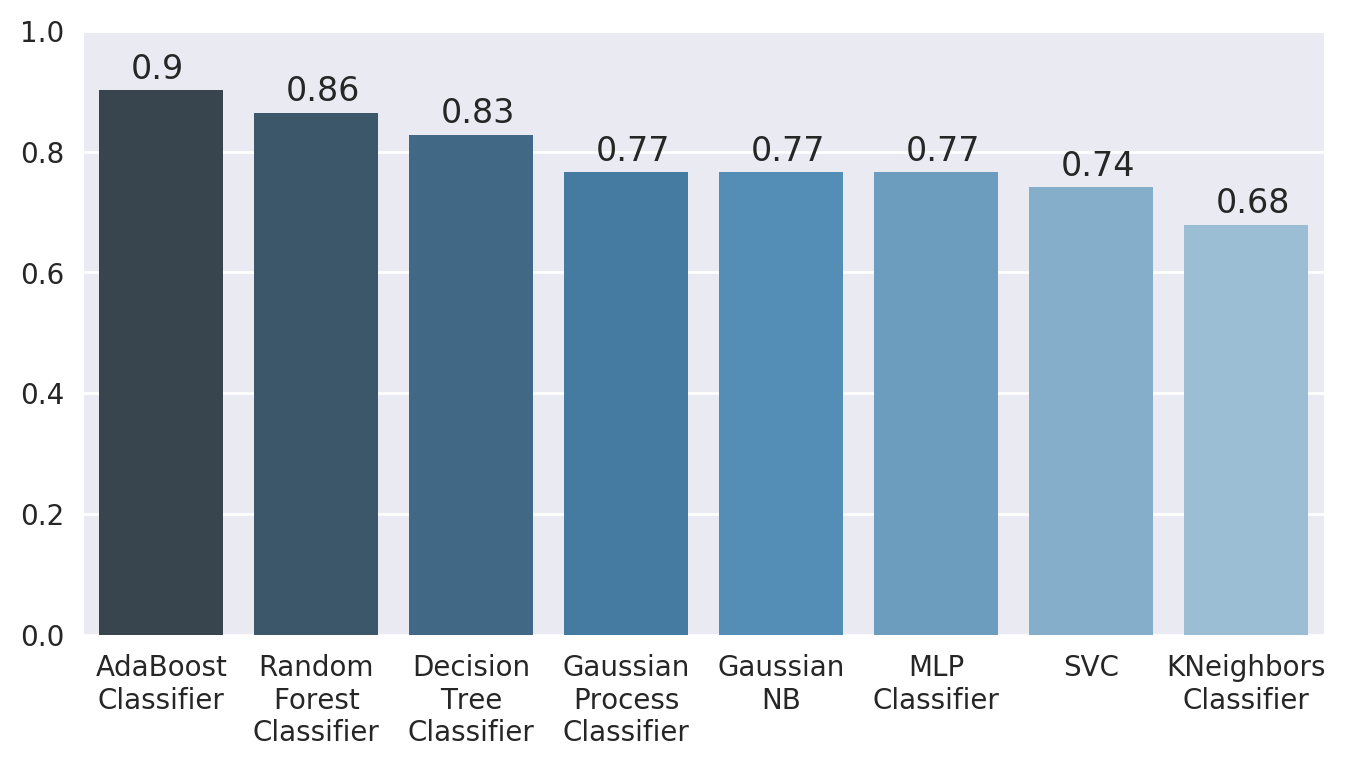
\includegraphics[width=\textwidth]{img/eval_law-case-model-selection}
\end{figure}

One can notice that the two included ensembles (AdaBoost and Random Forest) are the most successful.
Neural network (MLP) and Support Vector Machines (SVC) performed worse according to the expectation.
All estimators ran with default parameters as they are adjusted by Scikit learn library.

Undoubtedly, the AdaBoost Classifier outperformed all others, especially also the Random Forest.
However, during the parameter tunning of both of these two classifiers, the Random Forest achieved better performance when tuned than the AdaBoost.
Due to this finding, the final model is based on the Random Forest estimator.

\subsection{Keyword type selection}
% comparing keywords from case and doc to predict law-case
% Case....0.839 
% Doc ....0.863

\subsection{Layered architecture}
\label{eval:allinone-vs-features}
This experiment shows a comparison of two model architectures classifying case-related and law-related sentences.
One architecture consists of only one model, which analyses all attributes to predict class, whereas the second architecture is designed in two layers, where top-level model predicts class based on output of the underlying models.

The bottom-level models as well as the model in one-layer architecture are implemented by a neural network estimator with parameters as described in the section \ref{sec:bottom-level-nn}.
The top-level model is implemented by Random Forest classifier with 200 base estimators and 70 as maximal depth of a tree.
From the dataset of 263 documents, 40 case-related and 40 law-related were randomly selected to be the training set and the rest as testing set.
With sentences as data points, one has to be careful not to include sentences of a single document in both training and testing data.
Before the training process, the data sets were balanced in order to include the same number of sentences from both classes.
Therefore, baseline model would achieve $0.50$ accuracy.

The experiment was concluded in the following way.
For the \textit{All-in-one} architecture, the attributes were being consecutively appended to the vector that served as an input to the model.
The \textit{Separate} architecture, on the other hand, always trained bottom-level models on the individual attributes added so far, which output is used in the top-level model for predictions.
Thanks to this design, one can easily compare the two architectures with increasing number of attributes.

\begin{figure}[H]
\caption{Performance of all-in-one model (one layer) vs separate features (two layers)}
\label{fig:eval_all-in-one}
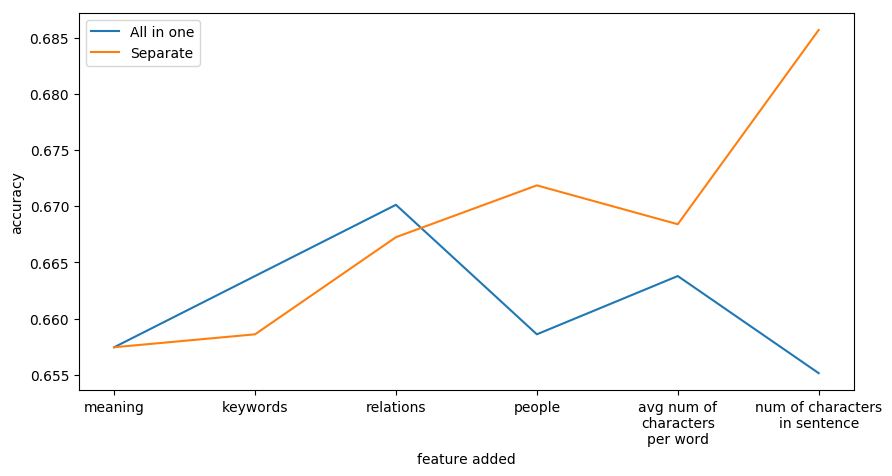
\includegraphics[width=\textwidth]{img/eval_all-in-one}
\end{figure}

The figure \ref{fig:eval_all-in-one} shows accuracies of the model architectures.
Notice that \textit{All-in-one} architecture is slightly more accurate up to the first three attributes; however, as the input vector prolongs, the ability to recognize patterns decreases.
The \textit{Separate} architecture has a disadvantage that the bottom-level models cannot cooperate together and extract the cross-information.
The advantage is that a few data is enough to train bottom-level models, and therefore the method scales better for increasing number of attributes.

% taky vysvetlit proc je uspesnost tak nizka - v originalnim pouzivame LOO - vic dat
The final table \ref{} shows higher accuracies, because instead of Leave One Out evaluation, here the Cross Validation is applied, which decreased the size of the training set. 
The accuracy is, however, significantly above the level of baseline (0.50), which means the outcome can be used as an argument for the decision to pick the layered architecture.

\subsection{Relations with types}
As described in the section \ref{sec:relation_embedding}, the relation consists of embedded words and types.
This experiment helped us confirm the theory, that the types are bringing a significant information value in classification of case-related and law-related documents.
Accuracy of a single model predicting classes of sentences achieved accuracy of $0.82$ with both types and words (dimension 758) and only $0.79$ with only words without the types (dimension 600).
The cross validation with stratified folds was applied to evaluate the result.
Based on this small test, all further experiments and final model includes relations with types.
% relations: acc with full vector with types: 82 \%, acc with only words (300+300) 79\% => types helps

\subsection{All words}
% predict law-case based on training on all 190k words, predict class of word - 0.83

\subsection{Word2vec contribution}
To show the contribution of \textit{Word2vec} embedding, this experiment compares it with the conventional one-hot embedding.
The accuracy score is computed for the same set of sentences, which were classified to the case-related and law-related by neural network explained in the section \ref{sec:bottom-level-nn}.

Since the data points are sentences and both embeddings encode words, the following technique were used to create one vector for each sentence.
The Word2vec embedding averaged the word vectors into one, and conventional embedding sums up the one-hot vectors to get a frequency vector.
As the unique number of words in all sentences is $11,019$, the frequency vectors are exactly that long.

\begin{figure}[h]
\caption{Performance of conventional embedding in one-hot vectors vs Word2vec embedding}
\label{fig:eval_word2vec_contribution}
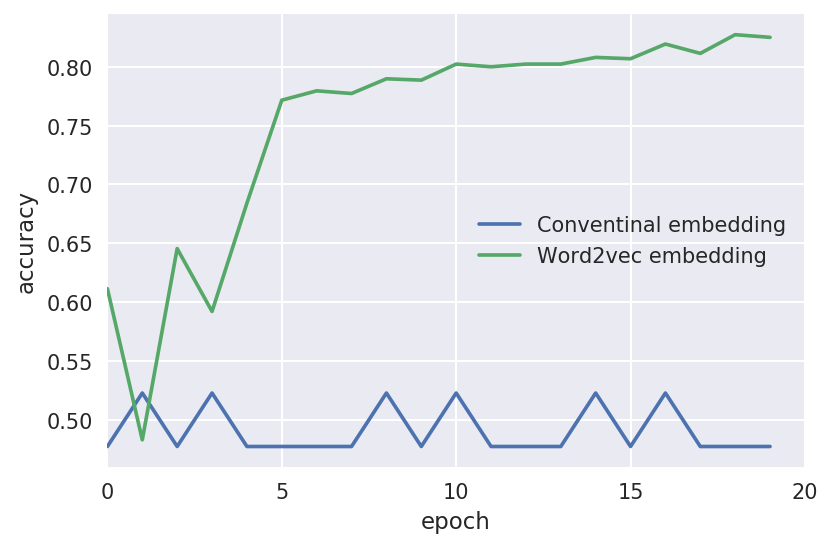
\includegraphics[width=\textwidth]{img/eval_word2vec_contribution}
\end{figure}

The figure \ref{fig:eval_word2vec_contribution} shows a very different learning curve of both models.
The accuracies were computed for a validation set (10\% of data) for each epoch of learning.
Whereas Word2vec embedding enables the model to learn new patterns systematically from fifth epoch, the conventional embedding undoubtedly lacks the ability to learn at all.
It is worth to note that this outcome is very specific for our type and number of data, as many other experiments with one-hot embeddings are successful.  
The conventional embedding is simply too large and sparse to deliver required amount of valuable information.


\section{Parameter tuning}

\subsection{Bottom-level Model}
\label{eval:bottom-model-tuning}
% tuning of the bottom-level NN, i.e. activation functions, optimizers and layers

\subsection{Law-Case Top-level Model}
\label{eval:law-case-model-tuning}
The outcome of the model selection in the section \ref{eval:law-case-model-selection} suggested Random Forests as the top-level model for predicting case-related and law-related documents. This section presents results from the parameter tunning.
Specifically, the number of estimators and maximum depth of decision trees were tuned.

\begin{figure}[h]
\caption{Parameter tunning of the Random Forest classifier for case-related or law-related classification}
\label{fig:eval_law-case-model-tunning}
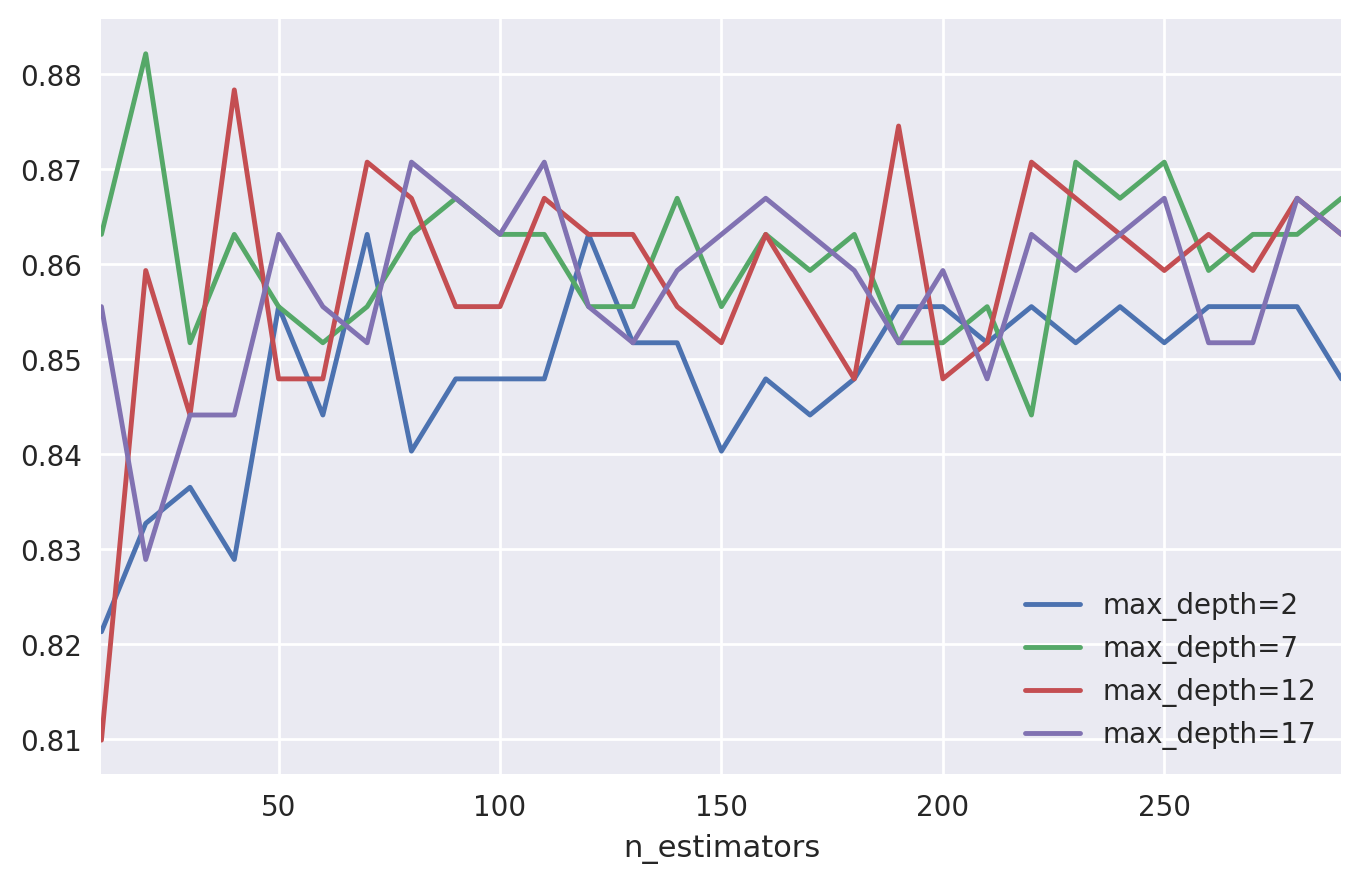
\includegraphics[width=\textwidth]{img/eval_law-case-model-tunning}
\end{figure}

The figure \ref{fig:eval_law-case-model-tunning} shows accuracy scores for different depths of trees.
The maximum level of 7 together with 20 estimators (individual decision trees) performed the best with 0.882, therefore these parameters were plugged in the final model.
Note that the tunning was performed with cross validation with 3 folds, which means the model was trained on only $2/3$ of data.
In case the model is trained on all but one document (Leave-One-Out), the accuracy is 0.890.

\section{Results}
% 1. print precision and recalls for all three relevances separately 
% 2. compare with the algorithm already in Legato - Hot Words
% 3. try evaluate some short passages from document and show concrete examples how it works


\chapter{Conclusion}

% future work
% - Watson NLU enables to create custom language model, which could recognize entities, keywords and relations even more precise if we feed it with legal data. We could not, since we have not enough text, but a future research could work with this.

% - Watson NLU enables 462 entities - possible to include all of them

% Matter of privacy - how to ensure the models do not enable to retrieve information about other case

% case lookup - find similar cases

% LSTM RNN networks - tried, but did not succeed, but maybe because not enough tunning

  \printbibliography[heading=bibintoc] %% Print the bibliography.

  \makeatletter\thesis@blocks@clear\makeatother
  \phantomsection %% Print the index and insert it into the
  \addcontentsline{toc}{chapter}{\indexname} %% table of contents.
  \printindex

\appendix %% Start the appendices.
\chapter{An appendix}
Here you can insert the appendices of your thesis.

\end{document}
